\documentclass[12pt, letterpaper]{article}

% --- Paquetes de configuración ---
\usepackage[utf8]{inputenc}
\usepackage[T1]{fontenc}
\usepackage[spanish, es-tabla]{babel} % Español
\usepackage{amsmath} % Para matemáticas avanzadas
\usepackage{geometry}
\geometry{left=3cm, right=3cm, top=3cm, bottom=3cm} % Márgenes estándar
\usepackage{graphicx} % Para imágenes
\usepackage{subcaption} % Para subfiguras lado a lado
\usepackage{float}    % Para posicionamiento exacto de figuras con [H]
\usepackage{tikz}     % Para el marco azul
\usetikzlibrary{calc}
\usepackage{enumitem} % Para listas personalizadas
\usepackage{hyperref} % Para enlaces en la ToC
\usepackage{titlesec} % Para formato de títulos
\usepackage{xltabular} % Para tablas que se dividen en varias páginas
\usepackage{ragged2e} % Para justificar texto en tablas

% --- Importar definiciones de métricas ---
% ============================================================================
% METRICS DEFINITIONS - CHAMPION MODEL (exp_05 XGBoost)
% Auto-generated from JSON metadata - DO NOT HARDCODE VALUES
% Last updated: 2026-04-15
% ============================================================================

% Cross-Validation Performance Metrics
\newcommand{\championROCAUC}{0.6391}
\newcommand{\championROCAUCstd}{0.0371}
\newcommand{\championBrierScore}{0.2672}

% Operating Point Performance Metrics (Test Set)
\newcommand{\championRecall}{0.8647}
\newcommand{\championSpecificity}{0.2854}
\newcommand{\championPrecision}{0.3634}
\newcommand{\championNPV}{0.8172}
\newcommand{\championFOneScore}{0.5118}
\newcommand{\championFTwoScore}{0.6778}
\newcommand{\championAccuracy}{0.4711}
\newcommand{\championKappa}{0.1100}
\newcommand{\championOptimalThreshold}{0.48}
\newcommand{\championAveragePrecision}{0.5171}

% Confusion Matrix Values
\newcommand{\championTP}{326}
\newcommand{\championFP}{571}
\newcommand{\championTN}{228}
\newcommand{\championFN}{51}
\newcommand{\championTPpct}{86.47}
\newcommand{\championFPpct}{71.46}
\newcommand{\championTNpct}{28.54}
\newcommand{\championFNpct}{13.53}

% Model Information
\newcommand{\championModelName}{XGBoost}
\newcommand{\championExperiment}{exp\_05\_hyperparameter\_search}

% Experiment Evolution - AUC-ROC Progression
\newcommand{\expOneAUC}{0.6153}
\newcommand{\expOneBestModel}{CatBoost}
\newcommand{\expTwoAUC}{0.6235}
\newcommand{\expTwoBestModel}{CatBoost}
\newcommand{\expThreeAUC}{0.6134}
\newcommand{\expThreeBestModel}{CatBoost}
\newcommand{\expFourAUC}{0.6209}
\newcommand{\expFourBestModel}{CatBoost}
\newcommand{\expFiveAUC}{0.6391}
\newcommand{\expFiveBestModel}{XGBoost}

% Top 3 Feature Importances (XGBoost exp_05)
\newcommand{\topFeatureOne}{SANGRADO\_MAYOR}
\newcommand{\topFeatureOneImportance}{19.16}
\newcommand{\topFeatureTwo}{HB\_x\_SANGRADO}
\newcommand{\topFeatureTwoImportance}{13.73}
\newcommand{\topFeatureThree}{DIABETES}
\newcommand{\topFeatureThreeImportance}{10.11}

% Clinical Interpretation
\newcommand{\recallInterpretation}{El modelo detecta \championRecall\ (\championTPpct\%) de los casos de choque hemorrágico}
\newcommand{\npvInterpretation}{Valor predictivo negativo de \championNPV, indicando alta confianza cuando predice ausencia de choque}


% Configuración de enlaces (sin recuadros rojos)
\hypersetup{
    colorlinks=true,
    linkcolor=black,
    filecolor=magenta,      
    urlcolor=blue,
}

% Configuración de párrafos
\setlength{\parskip}{0.5em}
\setlength{\parindent}{1cm}

% Configuración de títulos centrados (solo secciones)
\usepackage{sectsty}
\sectionfont{\centering}

% Configuración de altura de celdas en tablas
\renewcommand{\arraystretch}{1.5}

\begin{document}

% -----------------------------------------------------------------------------
% PÁGINA 1: PORTADA
% -----------------------------------------------------------------------------
\begin{titlepage}
    % Marco Azul usando TikZ
    \begin{tikzpicture}[remember picture, overlay]
        \draw[blue!90!black, line width=4pt] 
            ($(current page.north west) + (1.5cm,-1.5cm)$) 
            rectangle 
            ($(current page.south east) + (-1.5cm,1.5cm)$);
    \end{tikzpicture}

    \centering
    
    % Logotipo Universidad ICESI
    
\includegraphics[width=0.4\textwidth]{images/image001.png} 
    
    \vspace{2cm}
    
    {\Large \textbf{Predicción temprana de shock hemorrágico en pacientes sometidos a cirugía mayor no cardiaca mediante modelos de inteligencia artificial}}
    
    \vspace{1.5cm}
    
    {\Large \textbf{Proyecto de Grado}}
    
    \vspace{2cm}
    
    \textbf{Autores:}\\
    Cristian Eduardo Botina Carpio\\
    Juan Manuel Marín Angarita\\
    Óscar Andrés Gómez Lozano
    
    \vspace{1cm}
    
    \textbf{Tutores:}\\
    Ángela Villota Gómez
    
    \vfill
    
    \textbf{Universidad Icesi}\\
    Facultad Barberi de Ingeniería, Diseño y Ciencias Aplicadas\\
    Ingeniería de Sistemas\\
    Santiago De Cali\\
    2025
    
\end{titlepage}

% -----------------------------------------------------------------------------
% PÁGINA 2: TABLA DE CONTENIDO
% -----------------------------------------------------------------------------

\tableofcontents
\newpage

% -----------------------------------------------------------------------------
% PÁGINA 3: LISTA DE ACRÓNIMOS
% -----------------------------------------------------------------------------
\section*{Lista de acrónimos}
\addcontentsline{toc}{section}{Lista de acrónimos}

\begin{description}[style=multiline, leftmargin=3.5cm, font=\bfseries]
    \item[ACS] Sociedad \textbf{A}mericana de \textbf{C}irujanos (\textbf{A}merican \textbf{C}ollege of \textbf{S}urgeons)
    \item[AUC-ROC] \textbf{Á}rea \textbf{B}ajo la \textbf{C}urva ROC (\textbf{A}rea \textbf{U}nder the \textbf{R}eceiver \textbf{O}perating \textbf{C}haracteristic Curve)
    \item[CO] Gasto \textbf{C}ardíaco (\textbf{C}ardiac \textbf{O}utput)
    \item[CV] \textbf{V}alidación \textbf{C}ruzada (\textbf{C}ross \textbf{V}alidation)
    \item[DCS] \textbf{C}irugía de \textbf{C}ontrol de \textbf{D}año (\textbf{D}amage \textbf{C}ontrol \textbf{S}urgery)
    \item[DNN] \textbf{R}edes \textbf{N}euronales \textbf{P}rofundas (\textbf{D}eep \textbf{N}eural \textbf{N}etworks)
    \item[DT] \textbf{Á}rbol de \textbf{D}ecisión (\textbf{D}ecision \textbf{T}ree)
    \item[FC] \textbf{F}recuencia \textbf{C}ardíaca
    \item[FVL] \textbf{F}undación \textbf{V}alle de \textbf{L}ili
    \item[GBM] \textbf{M}áquina de \textbf{R}efuerzo de \textbf{G}radiente (\textbf{G}radient \textbf{B}oosting \textbf{M}achine)
    \item[IA] \textbf{I}nteligencia \textbf{A}rtificial
    \item[IMC] \textbf{Í}ndice de \textbf{M}asa \textbf{C}orporal
    \item[IS] \textbf{Í}ndice de \textbf{S}hock
    \item[KNN] \textbf{K} vecinos más cercanos (\textbf{K} \textbf{N}earest \textbf{N}eighbors)
    \item[LightGBM] \textbf{M}áquina de \textbf{R}efuerzo de \textbf{G}radiente \textbf{L}igera (\textbf{Light} \textbf{G}radient \textbf{B}oosting \textbf{M}achine)
    \item[ML] \textbf{A}prendizaje \textbf{A}utomático (\textbf{M}achine \textbf{L}earning)
    \item[MSI] \textbf{Í}ndice de \textbf{S}hock \textbf{M}odificado (\textbf{M}odified \textbf{S}hock \textbf{I}ndex)
    \item[NB] \textbf{N}aive \textbf{B}ayes (Clasificador probabilístico basado en el teorema de Bayes)
    \item[PAM] \textbf{P}resión \textbf{A}rterial \textbf{M}edia
    \item[PAS] \textbf{P}resión \textbf{A}rterial \textbf{S}istólica
    \item[PPH] \textbf{H}emorragia \textbf{P}ost\textbf{p}ancreatectomía (\textbf{P}ost\textbf{p}ancreatectomy \textbf{H}aemorrhage)
    \item[RPT] \textbf{R}esistencia \textbf{P}eriférica \textbf{T}otal
    \item[SHAP] E\textbf{x}plicaciones \textbf{A}ditivas de \textbf{S}hapley (\textbf{SH}apley \textbf{A}dditive ex\textbf{P}lanations)
    \item[SMOTE] Técnica de \textbf{S}obremuestreo de \textbf{M}inoría \textbf{S}intética (\textbf{S}ynthetic \textbf{M}inority \textbf{O}ver-sampling \textbf{TE}chnique)
    \item[THR] \textbf{R}esucitación \textbf{H}ipotensiva \textbf{T}itulada (\textbf{T}itrated \textbf{H}ypotensive \textbf{R}esuscitation)
    \item[TRIPOD] Informe \textbf{T}ransparente de un modelo de p\textbf{r}edicción mult\textbf{i}variable (\textbf{T}ransparent \textbf{R}eporting of a mult\textbf{i}variable \textbf{P}rediction model for Individual Prognosis \textbf{o}r \textbf{D}iagnosis)
    \item[UCI] \textbf{U}nidad de \textbf{C}uidados \textbf{I}ntensivos
    \item[VO] \textbf{V}ariable \textbf{O}bjetivo
    \item[VS] \textbf{V}olumen \textbf{S}anguíneo
\end{description}
\newpage

% -----------------------------------------------------------------------------
% PÁGINA 4: VACÍA
% -----------------------------------------------------------------------------
\mbox{}               
\newpage        

% -----------------------------------------------------------------------------
% PÁGINA 4: GLOSARIO
% -----------------------------------------------------------------------------
\section*{Glosario de términos}
\addcontentsline{toc}{section}{Glosario de términos}

\begin{description}[style=unboxed, leftmargin=0cm]
    \item[\textbf{Cirugía mayor no cardíaca:}] Procedimientos quirúrgicos extensos, de alta complejidad y duración, realizados fuera del sistema cardiovascular (por ejemplo, abdominales, ortopédicas mayores, oncológicas).
    
    \item[\textbf{Falla multiorgánica:}] Condición crítica en la que dos o más órganos vitales (como riñones, hígado, pulmones o corazón) dejan de funcionar adecuadamente, generalmente como consecuencia de un shock no tratado.
    
    \item[\textbf{Frecuencia cardíaca:}] Número de contracciones del corazón por minuto. Es un parámetro vital que aumenta (taquicardia) como mecanismo compensatorio ante la pérdida de volumen sanguíneo.
    
    \item[\textbf{Gasto cardíaco:}] Volumen total de sangre que el ventrículo izquierdo del corazón bombea hacia la aorta cada minuto. Se calcula como el producto de la frecuencia cardíaca por el volumen sistólico ($CO = FC \times VSistolico$).
    
    \item[\textbf{Hipovolemia:}] Estado patológico caracterizado por una reducción significativa del volumen de sangre circulante, que puede llevar a shock si no se corrige.
    
    \item[\textbf{Hipoperfusión tisular:}] Disminución del flujo sanguíneo hacia los tejidos, lo que impide el suministro adecuado de oxígeno y nutrientes, y la eliminación de desechos metabólicos. Es la base fisiopatológica del shock.
    
    \item[\textbf{Intervalo RR:}] Tiempo transcurrido entre dos ondas R consecutivas en un electrocardiograma. Su variabilidad es un indicador sensible de cambios en la función autonómica y puede anticipar eventos críticos.
    
    \item[\textbf{Perfusión tisular:}] Proceso mediante el cual la sangre, rica en oxígeno y nutrientes, es distribuida a través del sistema circulatorio para alcanzar todos los tejidos y órganos del cuerpo.
    
    \item[\textbf{Resistencia Periférica Total (RPT):}] Fuerza de oposición que encuentran los vasos sanguíneos (principalmente arteriolas) al flujo de la sangre. Es un determinante clave de la presión arterial junto con el gasto cardíaco.
    
    \item[\textbf{Shock hemorrágico:}] Tipo de shock hipovolémico causado específicamente por una pérdida aguda y significativa de volumen sanguíneo, que compromete la perfusión de órganos vitales y puede conducir a la muerte si no se trata.
    
    \item[\textbf{Taquicardia compensatoria:}] Respuesta fisiológica adaptativa en la que el corazón aumenta su frecuencia cardíaca para intentar mantener un gasto cardíaco adecuado y, por ende, la perfusión tisular, frente a una disminución del volumen sanguíneo.
\end{description}
\newpage

% -----------------------------------------------------------------------------
% PÁGINA 5: LISTA DE TABLAS E INICIO DE INTRODUCCIÓN
% -----------------------------------------------------------------------------
\listoftables
\addcontentsline{toc}{section}{Índice de tablas}
\newpage

% -----------------------------------------------------------------------------
% CONTENIDO PRINCIPAL
% -----------------------------------------------------------------------------

% -----------------------------------------------------------------------------
% 1. INTRODUCCIÓN
% -----------------------------------------------------------------------------
\section{Introducción}

\subsection{Contexto}

El shock hemorrágico es una falla aguda del sistema circulatorio, causada por una pérdida rápida del volumen sanguíneo, lo que impide mantener niveles suficientes de oxígeno para las funciones de órganos vitales. El shock postoperatorio tiene varios estados que progresan desde etapas compensadas hasta descompensación completa. Según Bonanno \cite{bonanno2023}, estos se dividen en cinco niveles que se basan en la respuesta fisiológica de paciente, donde en el nivel I están las personas que se encuentran en un estado de taquicardia leve y una presión arterial sistólica (PAS) en un rango nominal, mientras que en el nivel III se observa un aumento en la frecuencia cardiaca, disminución del PAS y pérdida de consciencia. La clasificación enfatiza el momento óptimo para intervenciones específicas (DCS y THR) en lugar de depender de umbrales fijos, de este modo adaptándose a datos del paciente como edad y comorbilidades. La mortalidad en etapas avanzadas (IV-V) se produce cuando se alcanza hipotensión extrema y signos evidentes de descompensación como pérdida absoluta de la consciencia, paro cardiaco, falla multiorgánica, etc. La detección temprana es crítica, ya que cada minuto de retraso aumenta el riesgo de muerte \cite{cannon2018}.

Actualmente el proceso de detección del shock hemorrágico conlleva evaluación completa de parte del personal médico, usando medidas como el índice de shock (IS), cociente que relaciona la taquicardia compensatoria con la caída de la presión arterial \cite{terceros2017}. Aunque el IS con punto de corte de 1,11 presenta una sensibilidad del 91,3\% y su versión modificada alcanza el 95,65\% de sensibilidad, ambos tienen limitaciones marcadas que dificultan el proceso de acción:

\begin{itemize}
    \item \textbf{Limitaciones de los índices convencionales:} Los métodos basados exclusivamente en presión arterial pueden no identificar hasta un 8--9\% de casos de hemorragia masiva en sus etapas iniciales \cite{terceros2017}.
    \item \textbf{Índices predictivos con sensibilidad y especificidad variables:}
    \begin{itemize}
        \item Shock Index (SI): Sensibilidad 91.3\%, especificidad 79.7\%.
        \item Modificado Shock Index (MSI): Sensibilidad 95.7\%, especificidad 75.8\%.
    \end{itemize}
    \item \textbf{Carga cognitiva del personal clínico:} La ``ceguera por desviación'' y la sobrecarga de información pueden afectar la toma de decisiones clínicas, especialmente en procedimientos prolongados.
    \item \textbf{Enfoque en manifestaciones avanzadas:} Los criterios diagnósticos habituales como la hipotensión se manifiestan en fases relativamente tardías del shock, lo que dificulta la intervención preventiva; no siempre se dispone de información individualizada sobre comorbilidades o características demográficas.
\end{itemize}

El retraso en la predicción temprana conlleva consecuencias serias que pueden repercutir en la salud del paciente, entre ellas:

\begin{itemize}
    \item Según \cite{cannon2018}, en Estados Unidos se registran más de 60.000 muertes anuales relacionadas con hemorragia; a nivel mundial, se estiman alrededor de 1,9 millones de muertes por año, de las cuales aproximadamente 1,5 millones se asocian a trauma físico.
    \item Aumento de transfusiones, infecciones, fallo multiorgánico y costos económicos.
\end{itemize}

La inteligencia artificial representa una herramienta complementaria prometedora para la detección temprana del shock hemorrágico, con el potencial de apoyar al equipo clínico en la identificación del denominado ``shock subclínico'', en el que ``la microcirculación subyacente se ve comprometida a pesar de que las variables de macrocirculación permanecen en rangos normales''. Los sistemas de monitoreo convencionales se centran principalmente en parámetros estáticos como la presión arterial, los cuales pueden mantenerse dentro de límites normales incluso cuando el paciente se aproxima al límite de su capacidad compensatoria, puesto que ``cualquier mecanismo compensatorio fisiológico tiene una respuesta máxima finita ante un estrés específico''.

Aunque herramientas como el índice de shock (SI) y el índice de shock modificado (MSI) han contribuido a mejorar la detección, presentan limitaciones en especificidad y no siempre contemplan la variabilidad individual en la respuesta compensatoria. Los modelos de machine learning ofrecen la posibilidad de complementar estos enfoques al integrar múltiples variables clínicas (hematocrito, tiempo quirúrgico, clasificación ASA, entre otros) y analizar sus interacciones complejas, permitiendo identificar patrones que resultan difíciles de procesar de forma simultánea durante la práctica clínica.

Sin embargo, estas soluciones aún enfrentan importantes limitaciones: la mayoría de los estudios existentes utilizan diseños retrospectivos con acceso limitado a datos temporales precisos, dependen de protocolos estandarizados en centros de alta volumetría que limitan su aplicabilidad en entornos menos especializados, y carecen de validación prospectiva en diversos escenarios clínicos. Además, la escasez de estudios prospectivos en el campo representa un obstáculo para la implementación clínica generalizada. La verdadera potencia de estos sistemas no radica en el reemplazo del personal, sino en la capacidad del sistema de generar alertas tempranas con parámetros interpretables y significativos para el tratamiento del paciente.

\subsection{Formulación del problema}

La detección tardía del shock hemorrágico en pacientes sometidos a cirugías mayores no cardiacas constituye un desafío crítico en la práctica clínica actual. En la mayoría de los casos, la identificación de esta complicación depende de la interpretación clínica del equipo médico y de criterios diagnósticos que frecuentemente se manifiestan en fases avanzadas de la condición, lo cual limita la capacidad de anticipación y aumenta la variabilidad en la toma de decisiones entre diferentes profesionales. Esta situación se ve agravada por la ausencia de protocolos estandarizados, la dificultad para interpretar cambios sutiles en los signos vitales y las limitaciones humanas en el monitoreo continuo durante procedimientos prolongados.

La consecuencia directa de esta detección tardía es un incremento en la mortalidad y morbilidad postoperatoria, con mayor riesgo de falla multiorgánica, complicaciones asociadas a transfusiones sanguíneas y recuperación prolongada de los pacientes. Asimismo, se generan impactos significativos en los recursos hospitalarios debido al aumento en la necesidad de transfusiones, cirugías adicionales, estancias prolongadas en UCI y sobrecarga del personal médico.

\subsection{Impacto del proyecto}

El proyecto tiene un impacto en el ámbito clínico, social e institucional. Desde el punto de vista clínico, la implementación del modelo permitirá reducir la mortalidad asociada a complicaciones relacionadas con shock hemorrágico, pues al anticipar este riesgo de forma temprana se puede evitar la falla multiorgánica, mejorando los resultados postoperatorios. Esto a su vez, contribuye al uso más eficiente de los recursos hospitalarios, ya que al disminuir la necesidad de estancias prolongadas en unidades de cuidados intensivos se logra una reducción en los costos, así como una mejor planificación de insumos como sangre y medicamentos.

Además, se promueve la innovación tecnológica en el sistema de salud de Colombia, que fortalece la colaboración entre las áreas de medicina e ingeniería e integra factores individuales del paciente. Esto transforma el paradigma del monitoreo, que actualmente funciona mediante una vigilancia basada en umbrales fijos y la experiencia del profesional de la salud, donde los indicadores no son lo suficientemente claros. Al predecir mediante un modelo el riesgo, se obtiene una estrategia más personalizada, dinámica y anticipatoria, especialmente importante en poblaciones de alto riesgo, donde la tolerancia a la hemorragia es mínima.

\subsection{Objetivo General}

Desarrollar y validar un modelo de inteligencia artificial que permita la predicción temprana del riesgo de shock hemorrágico en pacientes sometidos a cirugía mayor no cardiaca, integrando datos clínicos preoperatorios e intraoperatorios, con el fin de apoyar la toma de decisiones médicas oportunas y reducir complicaciones asociadas.

\subsection{Objetivos Específicos}

\begin{enumerate}[label=\alph*)]
    \item Construir un conjunto de datos estructurado a partir de registros clínicos preoperatorios e intraoperatorios, mediante procesos de limpieza, transformación y anonimización de la información.
    \item Definir los criterios clínicos y operativos para el diagnóstico de shock hemorrágico, estableciendo un marco consensuado con profesionales médicos y basado en literatura especializada.
    \item Identificar y caracterizar las variables clínicas más relevantes asociadas a la aparición de shock hemorrágico, considerando factores de riesgo individuales, comorbilidades y características demográficas.
    \item Entrenar y validar diferentes modelos de inteligencia artificial supervisados, evaluando su desempeño con métricas como sensibilidad, especificidad, F1-score, AUC-ROC y calibración.
    \item Diseñar y ejecutar un proceso de validación clínica inicial mediante la retroalimentación de expertos y/o la simulación de escenarios quirúrgicos históricos, con el fin de evaluar la aplicabilidad del modelo en un entorno real.
    \item Proponer una estrategia de integración del modelo predictivo en sistemas de información quirúrgica, contemplando aspectos técnicos, clínicos y de usabilidad para apoyar la toma de decisiones preventivas.
\end{enumerate}

\newpage

% -----------------------------------------------------------------------------
% 2. MARCO TEÓRICO

\newpage

\section{Marco Teórico}

En el contexto clínico, una presión arterial media (PAM) por debajo de 60 mmHg puede comprometer la perfusión tisular, es decir, el suministro de oxígeno a los órganos vitales. La PAM depende del gasto cardíaco (CO) y la resistencia periférica total (RPT), siendo el CO a su vez influenciado por el volumen sanguíneo y la frecuencia cardíaca. Cuando este equilibrio se rompe y se produce hipoperfusión, se desencadena un estado de shock. Según la American College of Surgeons (ACS), el shock se clasifica en cuatro tipos principales: cardiogénico, distributivo, obstructivo e hipovolémico \cite{hooper2022}. En particular, el shock hemorrágico es un tipo de shock hipovolémico que se produce por la pérdida de sangre \cite{cannon2018}, lo que puede llevar a la necrosis de las células tisulares, falla multiorgánica y muerte si no se trata a tiempo.

La clasificación del shock hemorrágico permite evaluar la gravedad de la pérdida sanguínea según los signos clínicos del paciente. La ACS identifica las siguientes 4 clases \cite{hooper2022}:

\begin{table}[H]
\centering
\caption{Clasificación del Shock Hipovolémico según la ACS}
\label{tab:clasificacion-shock}
\begin{tabular}{|l|l|l|l|l|}
\hline
\textbf{Clase} & \textbf{Volumen aprox.} & \textbf{Frecuencia Cardíaca} & \textbf{Presión Arterial} & \textbf{Estado mental} \\ \hline
I & <15\% & Normal & Normal & Ansioso \\ \hline
II & 15-30\% & 100 BPM a 120 BPM & Normal o leve & Inquieto \\ \hline
III & 30-40\% & Más de 120 BPM & Sistólica <90mmHg & Confuso \\ \hline
IV & >40\% & Más de 120 BPM & <60mmHg & Inconsciente \\ \hline
\end{tabular}
\end{table}

En cuanto a la fisiopatología del shock hemorrágico, este sigue una progresión definida. En sus fases iniciales, el sistema cardiovascular activa mecanismos homeostáticos como la taquicardia, vasoconstricción periférica y redistribución del flujo sanguíneo hacia el cerebro y corazón, esto con el fin de compensar la pérdida de sangre. Estos mecanismos, aunque permiten mantener una PAM estable durante las primeras etapas, genera un efecto máscara, donde el paciente parece estar estable hasta que ya se encuentra en una fase crítica. Un dato importante es que los signos clínicos mencionados anteriormente se suelen manifestar solo tras la pérdida de un 30-40\% del volumen circulante, lo que limita su capacidad para la detección temprana, caracterizada por hipotensión arterial, acidosis metabólica, coagulopatía y eventual colapso circulatorio.

Por otro lado, cambios sutiles en parámetros fisiológicos, como el intervalo RR en el electrocardiograma, desaturaciones intermitentes de oxígeno o tendencias en la presión arterial media pueden ser clave para anticipar a la descompensación clínica por minutos o incluso horas, pero son difíciles de identificar de forma continua por el personal médico, ya sea por sobrecarga cognitiva o fatiga durante procedimientos prolongados y la variabilidad en la interpretación clínica.

La Inteligencia Artificial (IA) aplicada a la predicción clínica se basa en el aprendizaje a partir de datos históricos, mediante modelos que identifican patrones complejos y predicen eventos futuros con un grado de incertidumbre cuantificable. En el contexto del shock hemorrágico, un modelo predictivo asigna una probabilidad de riesgo de que un paciente desarrolle esta condición crítica en los próximos minutos u horas, permitiendo intervenciones tempranas que pueden ser vitales. Para este fin, se han desarrollado diversos enfoques algorítmicos, cada uno con ventajas y limitaciones específicas según la naturaleza de los datos y los requisitos clínicos:

\begin{itemize}
    \item \textbf{Regresión logística con regularización Lasso:} la regresión logística es un modelo clásico para predicción binaria que estima la probabilidad de un evento mediante una función logística. Sin embargo, su principal limitación radica en la suposición de relaciones lineales entre las variables predictoras y el logaritmo de las probabilidades. Para superar parcialmente esta restricción y mejorar la interpretabilidad, se emplea la variante Lasso (Least Absolute Shrinkage and Selection Operator), que introduce una penalización L1 en la función de pérdida. Esta penalización fuerza a que algunos coeficientes se reduzcan exactamente a cero, lo que equivale a una selección automática de variables relevantes. Este enfoque no solo reduce la complejidad del modelo, sino que también mejora su capacidad de generalización, especialmente en escenarios con alta dimensionalidad o colinealidad entre predictores.

    \item \textbf{K-Nearest Neighbors (KNN):} este algoritmo no paramétrico clasifica o predice un resultado basándose en la similitud entre un nuevo caso y los k casos más cercanos en el espacio de características. Aunque KNN es intuitivo y no requiere suposiciones sobre la forma funcional de las relaciones, su desempeño depende críticamente de la elección de k, la métrica de distancia utilizada y la escala de las variables. En contextos clínicos, donde los datos pueden ser ruidosos o escasos, KNN puede volverse inestable si no se normalizan adecuadamente las variables o si el número de vecinos no se ajusta con validación cruzada rigurosa. No obstante, su simplicidad lo hace útil como modelo de referencia o en combinación con técnicas de reducción de dimensionalidad.

    \item \textbf{LightGBM (Light Gradient Boosting Machine):} como una implementación eficiente y escalable de los modelos de Gradient Boosting, LightGBM construye árboles de decisión de forma secuencial, donde cada nuevo árbol se entrena para corregir los errores residuales del modelo acumulado hasta ese punto. A diferencia de otros algoritmos de boosting, LightGBM utiliza una estrategia de crecimiento basada en hojas (leaf-wise) en lugar de niveles (level-wise), lo que le permite alcanzar mayor precisión con menor número de hojas. Además, incorpora técnicas como el muestreo basado en gradientes (Gradient-based One-Side Sampling, GOSS) y el agrupamiento exclusivo de características (Exclusive Feature Bundling, EFB), lo que reduce drásticamente el tiempo de entrenamiento y el uso de memoria sin sacrificar rendimiento. En entornos clínicos con grandes volúmenes de datos heterogéneos como señales vitales en tiempo real, laboratorios y antecedentes médicos, LightGBM ha demostrado ser particularmente eficaz para capturar interacciones no lineales y efectos de umbral, superando con frecuencia a modelos más simples en métricas de discriminación y calibración. El aprendizaje automático (ML), ha surgido como una herramienta clave en la medicina predictiva, permitiendo el análisis de grandes volúmenes de datos clínicos para identificar patrones que difícilmente serían vistos por un personal humano, aún con años de experiencia. A diferencia de los modelos estadísticos tradicionales, como regresión logística, los algoritmos de ML pueden manejar relaciones no lineales, lo que los hace mucho más adecuados para el contexto clínico, donde las relaciones son complejas.
\end{itemize}

Dado que la implementación de modelos de ML supone el uso de técnicas de caja negra, se utilizan técnicas para facilitar la interpretación:

\begin{itemize}
    \item \textbf{SHapley Additive exPlanations (SHAP):} esta técnica se basa en la teoría de juegos cooperativos de Shapley, asignando a cada variable un valor que representa su contribución marginal a la predicción final, considerando todas las posibles combinaciones de características. Los valores SHAP son coherentes, localmente exactos y aditivos, lo que permite no solo cuantificar la importancia global de una variable, sino también explicar predicciones individuales. En la práctica clínica, esto permite a los médicos ver, por ejemplo, que la presión arterial sistólica y la frecuencia cardíaca contribuyeron positivamente al riesgo de shock en un paciente específico, mientras que la saturación de oxígeno tuvo un efecto protector. Estas explicaciones facilitan la validación clínica del modelo y fomentan la adopción en la práctica real.

    \item \textbf{Local Interpretable Model-agnostic Explanations (LIME):} complementa a SHAP al aproximar localmente el comportamiento de un modelo complejo mediante un modelo interpretable (como una regresión lineal) en torno a una predicción individual. Esto permite generar explicaciones intuitivas por ejemplo, destacando las tres variables más influyentes en una alerta de alto riesgo, aunque con menor rigor teórico que SHAP. Ambas técnicas son compatibles con cualquier modelo (model-agnostic) y son ampliamente utilizadas en aplicaciones médicas para garantizar que las decisiones automatizadas sean auditables y clínicamente razonables.
\end{itemize}

Para validar que un modelo sea clínicamente útil debe seguir estándares de desarrollo, para esto existe la declaración Transparent Reporting of a multivariable Prediction model for Individual Prognosis or Diagnosis (TRIPOD) \cite{collins2015}, diseñada para garantizar transparencia, calidad y reproductibilidad, esencial para evaluar la generalización del modelo en distintas poblaciones y sistemas de salud.

\newpage

% -----------------------------------------------------------------------------
% 3. ESTADO DEL ARTE
% -----------------------------------------------------------------------------

\newpage

\section{Estado del Arte}

En los últimos años, el campo de la inteligencia artificial aplicada a la predicción de complicaciones postoperatorias ha experimentado un crecimiento significativo, siguen siendo pocos los estudios que destacan por sus resultados o procedimientos en la prevención del shock hemorrágico. Los modelos de ML surgen entonces como herramientas prometedoras para superar las limitaciones de los métodos tradicionales al integrar múltiples variables clínicas y proporcionar predicciones más precisas. Sin embargo, aún quedan desafíos metodológicos y prácticos que limitan su implementación clínica.

\subsection{Modelo predictivo para hemorragia pospancreatectomía}

Zhang et al.\ \cite{zhang2025} desarrollaron y validaron externamente un modelo de machine learning para la estratificación precisa del riesgo de hemorragia pospancreatectomía (PPH) mediante una cohorte internacional. El estudio utilizó una cohorte de entrenamiento de 3,609 pacientes de la base de datos del American College of Surgeons National Surgical Quality Improvement Program (ACS-NSQIP) y una cohorte de validación externa de 1,347 pacientes del National Cancer Center en China. Los investigadores compararon múltiples algoritmos evaluados, incluyendo GBM, Deep Neural Networks (DNN) y Logistic Regression, seleccionando finalmente el Lasso-GBM, el cual identificó predictores claves como: el índice de masa corporal (IMC), la clasificación ASA, la administración de esteroides preoperatorios, el uso de betabloqueadores, el tiempo quirúrgico y los niveles de hematocrito. Este enfoque usa regresión LASSO (Least Absolute Shrinkage and Selection Operator). Esta técnica es un modelo de IA que iterativamente penaliza las variables no esenciales, resuelve problemas de multicolinealidad y previene el overfitting. Sin embargo, presentó limitaciones importantes por la falta de datos temporales como el momento en el que comenzó la hemorragia y la dependencia de protocolos de centros de alta volumetría limitó su aplicabilidad en entornos menos estandarizados.

\subsection{Modelo predictivo para accidente cerebrovascular perioperatorio}

Cong et al.\ \cite{cong2025} desarrollaron y validaron un modelo basado en machine learning para predecir el riesgo de accidente cerebrovascular (stroke) perioperatorio en pacientes sometidos a cirugías no cardíacas, no vasculares y no neuroquirúrgicas. Utilizaron datos de 2,986 pacientes del Hospital Provincial de Henan, comparando nueve algoritmos diferentes de machine learning. El estudio desembocó en el uso de los modelos de LightGBM y KNN mostraron el mejor desempeño, con AUCs de 0.941 y 0.988 respectivamente en el conjunto de entrenamiento. Este estudio destacó por su manejo del desbalance de clases (solo el 16-20\% de los pacientes experimentaron stroke), utilizando métricas clínicas relevantes como sensibilidad y F1 Score. Además, incorporó SHAP para explicar las predicciones del modelo, facilitando la interpretación clínica. Sin embargo, el estudio y su enfoque en predicción preoperatoria no abordó la detección temprana postoperatoria que sería necesaria para intervenciones inmediatas.

\subsection{Predicción del recuperamiento de shock hemorrágico severo usando regresión logística}

Aunque la mayoría de los avances recientes en predicción de shock hemorrágico se han centrado en modelos clínicos con machine learning, algunos estudios preclínicos han explorado enfoques similares en modelos animales. En este caso, Lucas et al.\ \cite{lucas2019} desarrollaron un modelo de regresión logística con selección rigurosa de características que logró predecir la recuperación tras shock hemorrágico severo en ratas con una precisión del 84\%, superando a los métodos tradicionales basados únicamente en presión arterial y frecuencia cardíaca. Este enfoque metodológico, aunque no directamente aplicable en entornos clínicos humanos, refuerza el potencial de los modelos predictivos basados en múltiples parámetros fisiológicos para mejorar la toma de decisiones en situaciones críticas, lo que respalda la viabilidad de desarrollar sistemas similares adaptados al entorno postoperatorio humano.

\subsection{Modelos multimodales para pronóstico en UCI}

Pal et al.\ \cite{pal2022} presentaron ShockModes, un modelo multimodal para la predicción de resultados en UCI que integra tres fuentes de datos heterogéneas: notas clínicas de médicos procesadas con DocBERT (un Transformer entrenado en textos médicos), series temporales de signos vitales (frecuencia cardíaca, presión arterial, SpO\textsubscript{2}) procesadas con Regresión Logística, Random Forest, GradientBoost, AdaBoost y XGBoost, y datos de comorbilidades del paciente. El modelo alcanzó un recall de 0.81 y una especificidad de 0.94, demostrando el potencial de las arquitecturas multimodales en este dominio. Sin embargo, los propios autores reconocen que este enfoque requiere volúmenes de datos significativamente mayores y una infraestructura de recolección de datos más compleja que la disponible en la mayoría de centros clínicos. En nuestro caso, contamos únicamente con una de estas fuentes de datos (variables tabulares), lo que contextualiza las limitaciones de nuestro modelo en comparación con este referente.

\subsection{Limitaciones de los modelos predictivos clínicos}

Ma et al.\ \cite{ma2023} realizaron una revisión sistemática sobre el manejo deficiente de predictores continuos en modelos de predicción clínica. Su análisis reveló que la dicotomización de variables continuas (como convertir la edad o la hemoglobina en categorías binarias) y el uso de categorías arbitrarias para predictores continuos son prácticas extendidas que reducen significativamente la precisión predictiva de los modelos, al disminuir la información disponible sobre la verdadera distribución de cada variable. Esto es relevante para nuestro trabajo: los experimentos de categorización de EDAD y HB\_PREQX no produjeron mejoras y, de acuerdo con estos hallazgos, pudieron haber introducido pérdida de información.

Complementariamente, Steyerberg et al.\ \cite{steyerberg2018} analizaron las principales problemáticas de los enfoques de modelado tradicionales en contextos clínicos, identificando como riesgos críticos: el uso de datasets de tamaño reducido esperando generalización amplia, la categorización de predictores continuos, y la sobreestimación de los resultados del análisis estadístico (modelos que presentan resultados muy favorables en la evaluación interna pero que rinden significativamente peor en aplicación clínica real). Este último punto es especialmente pertinente en nuestro estudio, donde la optimización del umbral de decisión permitió mejorar el rendimiento en el conjunto de prueba a pesar de que los valores de la validación cruzada fueron moderados.

\subsection{Síntesis y brecha de conocimiento}

La revisión de estos estudios revela importantes avances metodológicos en la aplicación de machine learning para predecir complicaciones postoperatorias, pero también identifica una brecha crítica que aborda este proyecto: la ausencia de un sistema especializado para la detección temprana del shock hemorrágico postoperatorio en cirugía mayor no cardíaca. Mientras Zhang et al.\ \cite{zhang2025} desarrollaron un modelo predictivo para hemorragia pospancreatectomía y Cong et al.\ \cite{cong2025} se enfocaron en la predicción de stroke perioperatorio, ninguno aborda específicamente la detección temprana del shock hemorrágico en el período postoperatorio, cuando los signos clínicos pueden ser sutiles pero la intervención oportuna es crítica para la supervivencia. El estudio ShockModes \cite{pal2022} demuestra el potencial de las arquitecturas multimodales, pero requiere fuentes de datos heterogéneas que superan los datos disponibles en este proyecto. La brecha que aborda este proyecto es, por tanto, muy específica: desarrollar un sistema de alerta temprana basado en inteligencia artificial que permita identificar pacientes en riesgo de shock hemorrágico durante el período postoperatorio, reconociendo las limitaciones metodológicas señaladas por Ma et al.\ \cite{ma2023} y Steyerberg et al.\ \cite{steyerberg2018}.

\begin{table}[H]
\centering
\caption{Estado del arte en modelos predictivos para complicaciones postoperatorias}
\label{tab:estado-arte}
\small
\begin{tabular}{|p{2.5cm}|p{3cm}|p{4.5cm}|p{4.5cm}|}
\hline
\textbf{Proyecto} & \textbf{Temática principal} & \textbf{Metodología} & \textbf{Limitaciones} \\ \hline
Zhang et al.\ \cite{zhang2025} & Modelo predictivo para hemorragia pospancreatectomía & Modelo Lasso-GBM validado externamente; enfoque en explicabilidad clínica & Diseño retrospectivo restringió acceso a variables quirúrgicas detalladas; dependencia de protocolos de centros de alta volumetría \\ \hline
Cong et al.\ \cite{cong2025} & Modelo predictivo para stroke perioperatorio & LightGBM y KNN mostraron mejor desempeño (AUC 0.941 y 0.988); utilizó SHAP para explicabilidad clínica & Diseño retrospectivo con acceso limitado a variables quirúrgicas granulares; enfoque en predicción preoperatoria, no en detección temprana postoperatoria; no específico para shock hemorrágico \\ \hline
Lucas et al.\ \cite{lucas2019} & Predicción de recuperación tras shock hemorrágico severo mediante regresión logística & Regresión logística con selección rigurosa de características; evaluación de tres clasificadores: con todas las características, con conjunto reducido y solo MAP y HR & Precisión del 84\% en predicción de recuperación; modelo aplicado en contexto preclínico (ratas); no generalizable directamente a entornos clínicos humanos \\ \hline
Pal et al.\ \cite{pal2022} & Modelo multimodal para pronóstico en UCI (ShockModes) & Integración de notas clínicas (DocBERT), series temporales de signos vitales y comorbilidades; recall 0.81, especificidad 0.94 & Requiere múltiples fuentes de datos heterogéneas; infraestructura de recolección compleja; necesita volúmenes de datos mayores según los autores \\ \hline
Ma et al.\ \cite{ma2023}; Steyerberg et al.\ \cite{steyerberg2018} & Limitaciones metodológicas en modelos predictivos clínicos & Revisión sistemática de prácticas de modelado en regresión logística y validación interna & Categorizar predictores continuos reduce la precisión predictiva; datasets pequeños no garantizan generalización; sobreestimación de resultados estadísticos respecto al rendimiento clínico real \\ \hline
\end{tabular}
\end{table}

\newpage

% -----------------------------------------------------------------------------
% 4. METODOLOGÍA
% -----------------------------------------------------------------------------

\newpage

\section{Metodología}

El desarrollo del proyecto se basa en la integración de dos marcos metodológicos complementarios: CRISP-DM (Cross Industry Standard Process for Data Mining) \cite{crispdm1999}, ampliamente reconocido en el ámbito del análisis de datos e inteligencia artificial, y la guía TRIPOD (Transparent Reporting of a multivariable Prediction model for Individual Prognosis or Diagnosis) \cite{collins2015}, orientada a garantizar transparencia, reproducibilidad y rigor metodológico en el desarrollo de modelos predictivos clínicos.

El uso conjunto de ambos enfoques permite estructurar el proyecto desde una perspectiva técnico-científica, asegurando no solo la calidad del modelo, sino también su validez clínica y su potencial de integración en entornos hospitalarios.

\subsection{Fases metodológicas}

\textbf{Fase 1: Comprensión del problema y objetivos clínicos}

Corresponde a la formulación inicial del problema, el análisis del contexto clínico y la definición de los objetivos específicos del modelo predictivo. Durante esta fase se identifican los interesados principales (anestesiólogos, investigadores clínicos y especialistas en IA), los criterios de éxito clínico, así como las restricciones éticas y técnicas asociadas al manejo de datos sensibles. Esta fase se desarrolla siguiendo la primera etapa de CRISP-DM Business Understanding y las directrices iniciales de TRIPOD relativas a la definición clara del objetivo de predicción y la población de estudio. Se utiliza Microsoft Word para la documentación formal, Sharepoint para control colaborativo de versiones y Mendeley para la gestión de referencias.

\textbf{Fase 2: Comprensión y preparación de los datos}

En esta etapa se realiza el análisis exploratorio y la preparación del conjunto de datos proporcionado por la Fundación Valle del Lili (FVL), siguiendo las etapas Data Understanding y Data Preparation de CRISP-DM.

Las actividades incluyeron:

\begin{itemize}
    \item Exploración de distribución de variables clínicas y manejo de valores atípicos.
    \item Limpieza, transformación y codificación de variables categóricas y numéricas.
    \item Análisis de correlaciones y selección de variables relevantes con base en criterios clínicos y estadísticos.
\end{itemize}

De acuerdo con TRIPOD, en esta fase también se documentaron las características de la población, los métodos de adquisición de datos, los criterios de exclusión y el tratamiento de valores faltantes, garantizando la trazabilidad de los procedimientos. Las herramientas utilizadas son: Python (con librerías Pandas, NumPy, Matplotlib, Seaborn, entre otras) y Jupyter Notebook para el análisis exploratorio y la limpieza de datos; GitHub para control de versiones.

\textbf{Fase 3: Modelado y experimentación}

Esta fase corresponde a las etapas Modeling y Evaluation de CRISP-DM, y constituye el núcleo del trabajo actual. En ella se compararán distintos algoritmos de aprendizaje supervisado entre ellos Random Forest, Gradient Boosting (LightGBM) con el fin de determinar el modelo de mejor desempeño para la predicción temprana de shock hemorrágico.

Las actividades contempladas son:

\begin{itemize}
    \item División del dataset en conjuntos de entrenamiento, validación y prueba.
    \item Ajuste de hiperparámetros mediante validación cruzada estratificada.
    \item Evaluación del desempeño con métricas clínicas: sensibilidad, especificidad, F1-score, AUC-ROC y calibración, con enfoque en alta sensibilidad
    \item Interpretabilidad del modelo mediante técnicas SHAP para garantizar la transparencia y la validación clínica de los resultados.
\end{itemize}

Desde la perspectiva TRIPOD, esta fase incluye la documentación exhaustiva del proceso de modelado, el método de validación interna y el análisis de robustez y sesgos.

\textbf{Fase 4: Validación clínica preliminar}

En esta etapa se realiza una evaluación preliminar del modelo junto con expertos médicos, utilizando escenarios quirúrgicos históricos simulados. El propósito es verificar la coherencia clínica de las predicciones y la aplicabilidad práctica del modelo en entornos reales.

Esta fase sigue las recomendaciones TRIPOD sobre validación y reporte de resultados, incluyendo:

\begin{itemize}
    \item Identificación de limitaciones y posibles fuentes de sesgo.
    \item Elaboración de tablas y figuras explicativas conforme a los lineamientos de reporte TRIPOD.
\end{itemize}

\textbf{Fase 5: Despliegue y Documentación final}

Se consolida la documentación técnica y científica del proyecto, incluyendo el informe final, las visualizaciones de resultados y los anexos de código reproducible. En este caso, no se integrará el modelo con los sistemas de FVL, pero se busca realiza la etapa Deployment de CRISP-DM con versionamiento de modelos.

\newpage

% -----------------------------------------------------------------------------
% 5. DESARROLLO DE LA PROPUESTA
% -----------------------------------------------------------------------------

\newpage

\section{Desarrollo de la propuesta}

\subsection{Estrategia experimental}

La etapa experimental se estructuro en cinco experimentos secuenciales: \textit{baseline}, \textit{agregaciones}, \textit{categorizaciones}, \textit{pruning} e \textit{hiperparametros}. Esta nomenclatura coincide con el flujo de experimentacion definido para la sustentacion.

Todas las metricas reportadas en esta seccion se obtienen directamente de los metadatos generados por el pipeline, usando como fuente primaria:

\begin{itemize}
\item \texttt{doc/experiments/tmp\_metrics\_summary.tsv} para metricas consolidadas por experimento y modelo.
\item \texttt{doc/experiments/exp\_05\_hyperparameter\_search/models/<modelo>/plots/plot\_metadata.json} para metricas operativas detalladas del duelo final.
\end{itemize}

\subsection{Experimento 1: Baseline}

En el experimento baseline se evaluaron siete algoritmos con configuracion base para establecer la linea de referencia.

\begin{table}[H]
\centering
\caption{Top 3 modelos por AUC-ROC en el Experimento 1}
\label{tab:exp1-top3}
\begin{tabular}{|l|c|}
\hline
\textbf{Modelo} & \textbf{AUC-ROC} \\ \hline
catboost & 0.6153 \\ \hline
logistic\_regression\_lasso & 0.6055 \\ \hline
xgboost & 0.5950 \\ \hline
\end{tabular}
\end{table}

\begin{figure}[H]
\centering
\begin{subfigure}[b]{0.48\textwidth}
\centering

\includegraphics[width=\textwidth]{../experiments/exp_01_base_models/comparison_plots/roc_comparison.png}
\caption{Comparacion ROC global}
\label{fig:exp1-roc}
\end{subfigure}
\hfill
\begin{subfigure}[b]{0.48\textwidth}
\centering
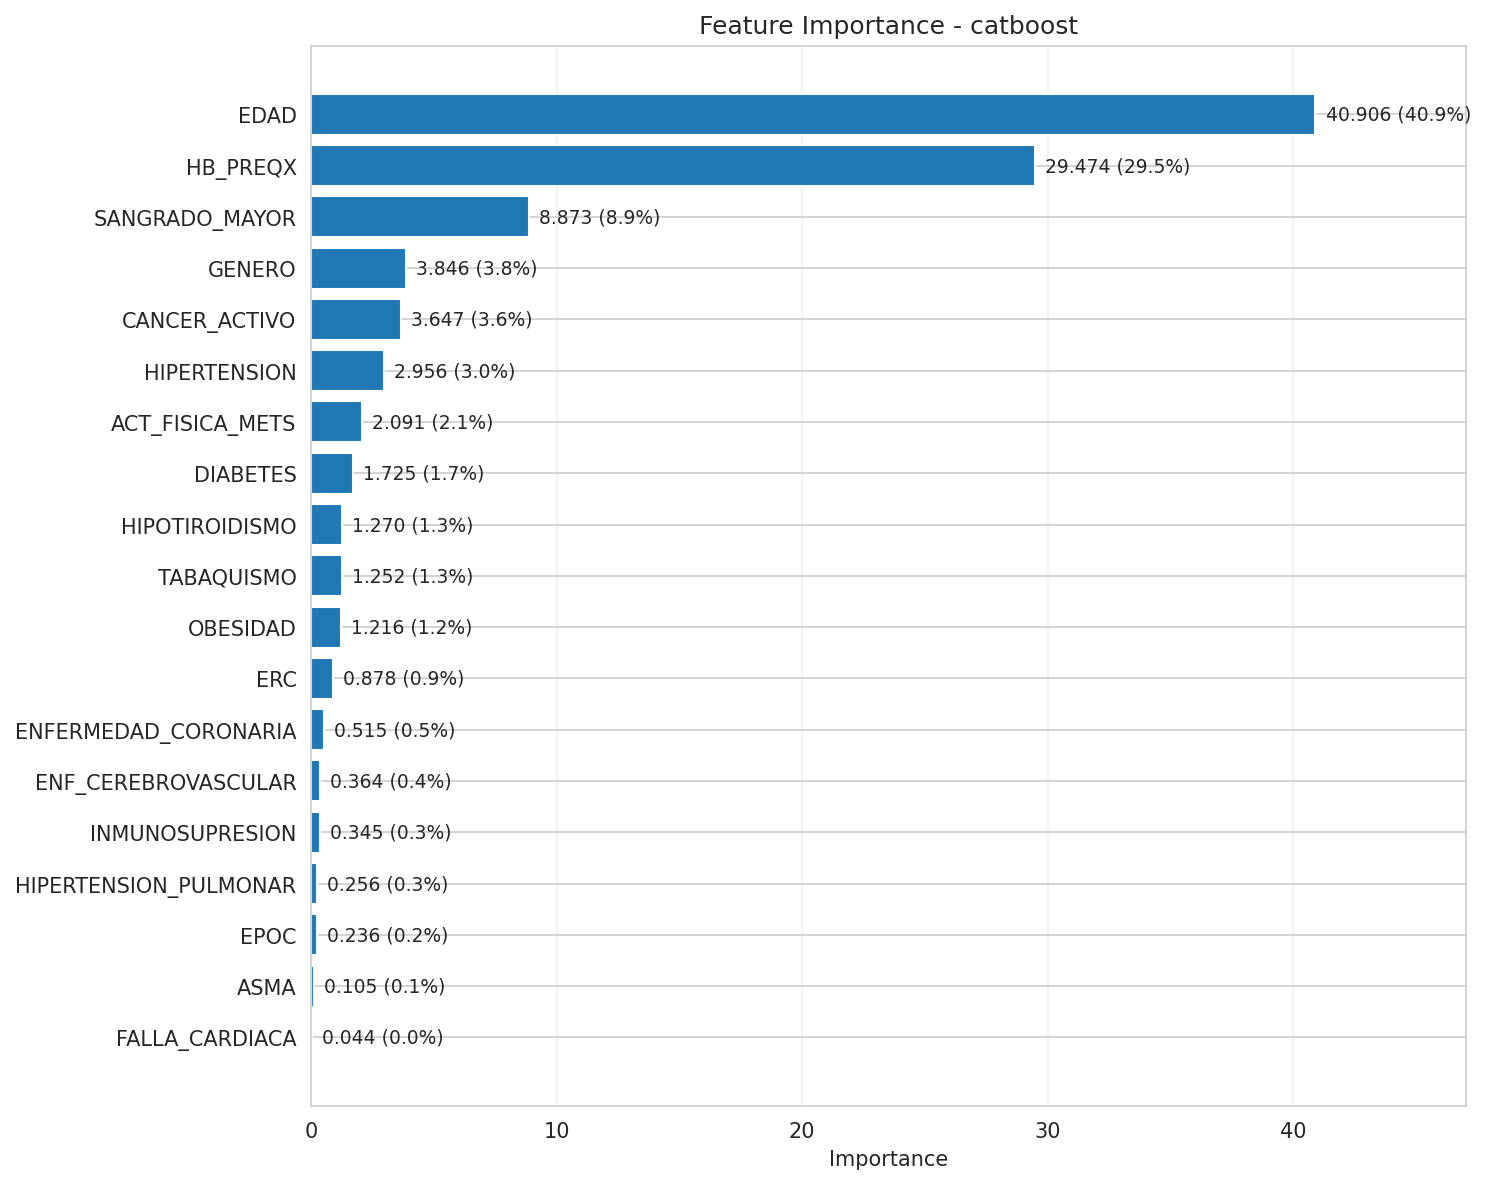
\includegraphics[width=\textwidth]{../experiments/exp_01_base_models/models/catboost/plots/feature_importance.png}
\caption{Importancia variables (catboost)}
\label{fig:exp1-fi-catboost}
\end{subfigure}
\caption{Resultados Experimento 1}
\label{fig:exp1-results}
\end{figure}

\subsection{Experimento 2: Agregaciones}

Se incorporaron variables derivadas y agregaciones clinicas para aumentar la capacidad discriminativa del modelo. El mejor resultado de esta fase fue catboost con AUC-ROC de 0.6192.

\begin{table}[H]
\centering
\caption{Top 3 modelos por AUC-ROC en el Experimento 2}
\label{tab:exp2-top3}
\begin{tabular}{|l|c|}
\hline
\textbf{Modelo} & \textbf{AUC-ROC} \\ \hline
catboost & 0.6192 \\ \hline
logistic\_regression\_lasso & 0.6055 \\ \hline
xgboost & 0.6045 \\ \hline
\end{tabular}
\end{table}

\begin{figure}[H]
\centering
\begin{subfigure}[b]{0.48\textwidth}
\centering

\includegraphics[width=\textwidth]{../experiments/exp_02_aggregated_features/comparison_plots/roc_comparison.png}
\caption{Comparacion ROC global}
\label{fig:exp2-roc}
\end{subfigure}
\hfill
\begin{subfigure}[b]{0.48\textwidth}
\centering

\includegraphics[width=\textwidth]{../experiments/exp_02_aggregated_features/models/catboost/plots/feature_importance.png}
\caption{Importancia variables (catboost)}
\label{fig:exp2-fi-catboost}
\end{subfigure}
\caption{Resultados Experimento 2}
\label{fig:exp2-results}
\end{figure}

\subsection{Experimento 3: Categorizaciones}

Se evaluo la categorizacion de variables continuas en rangos clinicos. El resultado mostro una caida frente al experimento anterior, con mejor AUC-ROC de 0.6134 (catboost), lo cual sugiere perdida de informacion discriminativa al discretizar.

\begin{table}[H]
\centering
\caption{Top 3 modelos por AUC-ROC en el Experimento 3}
\label{tab:exp3-top3}
\begin{tabular}{|l|c|}
\hline
\textbf{Modelo} & \textbf{AUC-ROC} \\ \hline
catboost & 0.6134 \\ \hline
logistic\_regression\_lasso & 0.6037 \\ \hline
xgboost & 0.5950 \\ \hline
\end{tabular}
\end{table}

\begin{figure}[H]
\centering

\includegraphics[width=0.85\textwidth]{../experiments/exp_03_categorical_features/comparison_plots/roc_comparison.png}
\caption{Comparacion ROC global del Experimento 3}
\label{fig:exp3-roc}
\end{figure}

% \begin{figure}[H]
% \centering
% 
\includegraphics[width=0.78\textwidth]{../experiments/exp_03_categorical_features/models/catboost/plots/feature_importance.png}
% \caption{Importancia de variables del modelo lider (catboost) en el Experimento 3}
% \label{fig:exp3-fi-catboost}
% \end{figure}
% Nota: Grafica de importancia de variables omitida debido a archivo corrupto

\subsection{Experimento 4: Pruning}

La cuarta fase se enfoco en reducir ruido y mantener solo caracteristicas con mayor utilidad predictiva. Se descartaron siete variables de baja ocurrencia (criterio minimo: 10 casos) que mostraron aporte marginal al desempeno discriminativo en fases previas.

\begin{table}[H]
\centering
\caption{Variables descartadas en feature pruning}
\label{tab:exp4-pruned-vars}
\begin{tabular}{|l|}
\hline
\textbf{Variable} \\ \hline
ENFERMEDAD\_CORONARIA \\ \hline
FALLA\_CARDIACA \\ \hline
INMUNOSUPRESION \\ \hline
HIPERTENSION\_PULMONAR \\ \hline
EPOC \\ \hline
ASMA \\ \hline
ENF\_CEREBROVASCULAR \\ \hline
\end{tabular}
\end{table}

Tras la eliminacion de estas variables, catboost volvio a liderar con AUC-ROC de 0.6237, manteniendo resultados competitivos con un conjunto de caracteristicas mas compacto.

\begin{table}[H]
\centering
\caption{Top 4 modelos por AUC-ROC en el Experimento 4}
\label{tab:exp4-top4}
\begin{tabular}{|l|c|}
\hline
\textbf{Modelo} & \textbf{AUC-ROC} \\ \hline
catboost & 0.6237 \\ \hline
logistic\_regression\_lasso & 0.6067 \\ \hline
xgboost & 0.6038 \\ \hline
lightgbm & 0.5995 \\ \hline
\end{tabular}
\end{table}

\begin{figure}[H]
\centering
\begin{subfigure}[b]{0.48\textwidth}
\centering

\includegraphics[width=\textwidth]{../experiments/exp_04_feature_pruning/comparison_plots/roc_comparison.png}
\caption{Comparacion ROC global}
\label{fig:exp4-roc}
\end{subfigure}
\hfill
\begin{subfigure}[b]{0.48\textwidth}
\centering

\includegraphics[width=\textwidth]{../experiments/exp_04_feature_pruning/models/catboost/plots/roc_curve_cv.png}
\caption{ROC CV catboost (lider)}
\label{fig:exp4-catboost-roc}
\end{subfigure}
\caption{Resultados Experimento 4}
\label{fig:exp4-results}
\end{figure}

\subsubsection{Comparativa complementaria en pruning}

Para reproducir el analisis de la presentacion, se incorpora la comparativa visual de curvas ROC en CV para los contendientes logistic\_regression\_lasso y xgboost bajo el mismo esquema de poda.

\begin{figure}[H]
\centering
\begin{subfigure}[b]{0.48\textwidth}
\centering

\includegraphics[width=\textwidth]{../experiments/exp_04_feature_pruning/models/logistic_regression_lasso/plots/roc_curve_cv.png}
\caption{Logistic Regression Lasso}
\label{fig:exp4-lasso-roc}
\end{subfigure}
\hfill
\begin{subfigure}[b]{0.48\textwidth}
\centering

\includegraphics[width=\textwidth]{../experiments/exp_04_feature_pruning/models/xgboost/plots/roc_curve_cv.png}
\caption{XGBoost}
\label{fig:exp4-xgb-roc}
\end{subfigure}
\caption{Curvas ROC en CV - Comparativa complementaria Experimento 4}
\label{fig:exp4-roc-comp}
\end{figure}

\subsection{Experimento 5: Hiperparametros}

La fase final realizo optimizacion de hiperparametros para todos los modelos y consolido la comparacion final de desempeno.

\begin{table}[H]
\centering
\caption{Ranking de modelos por AUC-ROC en el Experimento 5}
\label{tab:exp5-ranking}
\begin{tabular}{|c|l|c|}
\hline
\textbf{Ranking} & \textbf{Modelo} & \textbf{AUC-ROC} \\ \hline
1 & random\_forest & 0.6404 \\ \hline
2 & lightgbm & 0.6384 \\ \hline
3 & xgboost & 0.6371 \\ \hline
4 & decision\_tree & 0.6354 \\ \hline
5 & catboost & 0.6215 \\ \hline
6 & logistic\_regression\_lasso & 0.6068 \\ \hline
7 & naive\_bayes & 0.5707 \\ \hline
\end{tabular}
\end{table}

\begin{figure}[H]
\centering
\begin{subfigure}[b]{0.48\textwidth}
\centering

\includegraphics[width=\textwidth]{../experiments/exp_05_hyperparameter_search/comparison_plots/roc_comparison.png}
\caption{Comparacion ROC global}
\label{fig:exp5-roc}
\end{subfigure}
\hfill
\begin{subfigure}[b]{0.48\textwidth}
\centering

\includegraphics[width=\textwidth]{../experiments/exp_05_hyperparameter_search/comparison_plots/roc_boxplot_comparison.png}
\caption{Distribucion AUC-ROC CV}
\label{fig:exp5-roc-boxplot}
\end{subfigure}
\caption{Desempeno comparativo Experimento 5}
\label{fig:exp5-performance}
\end{figure}

\begin{figure}[H]
\centering

\includegraphics[width=0.78\textwidth]{../experiments/exp_05_hyperparameter_search/models/random_forest/plots/feature_importance.png}
\caption{Importancia de variables del modelo lider (random\_forest) en el Experimento 5}
\label{fig:exp5-rf-fi}
\end{figure}

\subsubsection{Comparativa final: Random Forest vs Decision Tree}

Para la decision final se contrasto el mejor modelo discriminativo (random\_forest) frente al mejor candidato interpretable (decision\_tree), usando las metricas de operacion reportadas en \texttt{plot\_metadata.json}.

\begin{table}[H]
\centering
\caption{Comparativa de metricas operativas en el Experimento 5}
\label{tab:exp5-duelo}
\begin{tabular}{|l|c|c|}
\hline
\textbf{Metrica} & \textbf{random\_forest} & \textbf{decision\_tree} \\ \hline
AUC-ROC (CV) & 0.6404 & 0.6354 \\ \hline
Threshold optimo & 0.38 & 0.22 \\ \hline
Recall & 0.8196 & 0.8568 \\ \hline
Specificity & 0.3567 & 0.3154 \\ \hline
Precision & 0.3755 & 0.3713 \\ \hline
NPV & 0.8074 & 0.8235 \\ \hline
F1-score & 0.5150 & 0.5180 \\ \hline
F2-score & 0.6628 & 0.6791 \\ \hline
Accuracy & 0.5051 & 0.4889 \\ \hline
Kappa & 0.1344 & 0.1280 \\ \hline
\end{tabular}
\end{table}

Desde el criterio clinico de deteccion temprana, random\_forest se prioriza por mayor AUC-ROC y mejor balance recall-especificidad. En paralelo, decision\_tree conserva valor practico por su transparencia estructural y mayor interpretabilidad para discusion con equipo medico.

\begin{figure}[H]
\centering
\begin{subfigure}[b]{0.48\textwidth}
\centering

\includegraphics[width=\textwidth]{../experiments/exp_05_hyperparameter_search/models/random_forest/plots/roc_curve_cv.png}
\caption{Random Forest (AUC=0.6404)}
\label{fig:exp5-rf-roc}
\end{subfigure}
\hfill
\begin{subfigure}[b]{0.48\textwidth}
\centering

\includegraphics[width=\textwidth]{../experiments/exp_05_hyperparameter_search/models/decision_tree/plots/roc_curve_cv.png}
\caption{Decision Tree (AUC=0.6354)}
\label{fig:exp5-tree-roc}
\end{subfigure}
\caption{Curvas ROC en CV - Experimento 5}
\label{fig:exp5-roc-comp}
\end{figure}

\subsubsection{Estructura e interpretacion del arbol de decision}

El modelo \texttt{decision\_tree} optimizado genera un clasificador binario con profundidad maxima de 7 niveles y 27 hojas terminales. La figura \ref{fig:exp5-tree-structure} presenta la estructura completa del arbol.

\begin{figure}[H]
\centering

\includegraphics[width=0.98\textwidth]{../experiments/exp_05_hyperparameter_search/models/decision_tree/plots/decision_tree_full.png}
\caption{Estructura completa del arbol de decision optimizado (Experimento 5)}
\label{fig:exp5-tree-structure}
\end{figure}

\textbf{Analisis de la estructura de decision:}

\begin{itemize}
\item \textbf{Configuracion general:} Clasificador binario basado en criterio de Gini. La Clase 0.0 (naranja, shock ausente) representa el 67.9\% de casos en el nodo raiz. La Clase 1.0 (azul, shock presente) se concentra en ramas especificas de la derecha del arbol.

\item \textbf{Variables con mayor poder discriminativo:} \texttt{SANGRADO\_MAYOR} actua como variable de division en el nodo raiz (critica para identificacion temprana). \texttt{EDAD} modula la probabilidad de shock en ambas ramas principales. \texttt{HB\_PREQX} y \texttt{SINDROME\_METABOLICO} refinan la clasificacion en nodos internos.

\item \textbf{Logica de decision principal:} La rama de \texttt{SANGRADO\_MAYOR} $> 1.582$ constituye la ruta critica para identificar casos de shock (Clase 1.0), especialmente cuando se combina con \texttt{EDAD} $> 0.236$ (Z-score estandarizado), generando alta pureza de clase positiva. Si el sangrado es $\leq 1.582$, la probabilidad de shock es minima ($<$ 0.20), salvo interacciones especificas entre edad y hemoglobina preoperatoria.

\item \textbf{Perfil de riesgo maximo:} El riesgo mas alto de shock (Clase 1.0) se concentra en pacientes con valores altos de sangrado intraoperatorio (Z-score $> 1.582$) y edades especificas: mayores de 65 anos (Z-score $> 0.236$) o en rango medio de 50-65 anos (Z-score entre $-0.877$ y $0.236$). La combinacion de estas condiciones eleva la probabilidad de shock por encima del 60\% en hojas terminales especificas.
\end{itemize}

\subsubsection{Comparativas visuales del duelo final}

Adicionalmente se incluyen las mismas comparativas visuales presentadas en sustentacion para contrastar estabilidad y comportamiento operativo entre random\_forest y decision\_tree.

\begin{figure}[H]
\centering
\begin{subfigure}[b]{0.48\textwidth}
\centering

\includegraphics[width=\textwidth]{../experiments/exp_05_hyperparameter_search/models/random_forest/plots/cv_fold_plots/cv_fold_roc_auc.png}
\caption{Random Forest}
\label{fig:exp5-rf-cv-box}
\end{subfigure}
\hfill
\begin{subfigure}[b]{0.48\textwidth}
\centering

\includegraphics[width=\textwidth]{../experiments/exp_05_hyperparameter_search/models/decision_tree/plots/cv_fold_plots/cv_fold_roc_auc.png}
\caption{Decision Tree}
\label{fig:exp5-tree-cv-box}
\end{subfigure}
\caption{Boxplot de AUC-ROC por fold en CV - Experimento 5}
\label{fig:exp5-cv-boxplot-comp}
\end{figure}

\begin{figure}[H]
\centering
\begin{subfigure}[b]{0.48\textwidth}
\centering

\includegraphics[width=\textwidth]{../experiments/exp_05_hyperparameter_search/models/random_forest/plots/perf_precision_npv.png}
\caption{Random Forest}
\label{fig:exp5-rf-precision-npv}
\end{subfigure}
\hfill
\begin{subfigure}[b]{0.48\textwidth}
\centering

\includegraphics[width=\textwidth]{../experiments/exp_05_hyperparameter_search/models/decision_tree/plots/perf_precision_npv.png}
\caption{Decision Tree}
\label{fig:exp5-tree-precision-npv}
\end{subfigure}
\caption{Comparativa Precision-NPV - Experimento 5}
\label{fig:exp5-precision-npv-comp}
\end{figure}

\begin{figure}[H]
\centering
\begin{subfigure}[b]{0.48\textwidth}
\centering

\includegraphics[width=\textwidth]{../experiments/exp_05_hyperparameter_search/models/random_forest/plots/perf_f1_f2.png}
\caption{Random Forest}
\label{fig:exp5-rf-f1-f2}
\end{subfigure}
\hfill
\begin{subfigure}[b]{0.48\textwidth}
\centering

\includegraphics[width=\textwidth]{../experiments/exp_05_hyperparameter_search/models/decision_tree/plots/perf_f1_f2.png}
\caption{Decision Tree}
\label{fig:exp5-tree-f1-f2}
\end{subfigure}
\caption{Comparativa F1-F2 - Experimento 5}
\label{fig:exp5-f1-f2-comp}
\end{figure}

\begin{figure}[H]
\centering
\begin{subfigure}[b]{0.48\textwidth}
\centering

\includegraphics[width=\textwidth]{../experiments/exp_05_hyperparameter_search/models/random_forest/plots/kappa.png}
\caption{Random Forest}
\label{fig:exp5-rf-kappa}
\end{subfigure}
\hfill
\begin{subfigure}[b]{0.48\textwidth}
\centering

\includegraphics[width=\textwidth]{../experiments/exp_05_hyperparameter_search/models/decision_tree/plots/kappa.png}
\caption{Decision Tree}
\label{fig:exp5-tree-kappa}
\end{subfigure}
\caption{Comparativa Kappa - Experimento 5}
\label{fig:exp5-kappa-comp}
\end{figure}

\begin{figure}[H]
\centering
\begin{subfigure}[b]{0.48\textwidth}
\centering

\includegraphics[width=\textwidth]{../experiments/exp_05_hyperparameter_search/models/random_forest/plots/confusion_matrix_normalized.png}
\caption{Random Forest}
\label{fig:exp5-rf-confusion}
\end{subfigure}
\hfill
\begin{subfigure}[b]{0.48\textwidth}
\centering

\includegraphics[width=\textwidth]{../experiments/exp_05_hyperparameter_search/models/decision_tree/plots/confusion_matrix_normalized.png}
\caption{Decision Tree}
\label{fig:exp5-tree-confusion}
\end{subfigure}
\caption{Matriz de confusion normalizada - Experimento 5}
\label{fig:exp5-confusion-comp}
\end{figure}

\subsection{Evolucion global y cierre de fase experimental}

\begin{table}[H]
\centering
\caption{Evolucion del mejor AUC-ROC por experimento}
\label{tab:evolucion-auc}
\begin{tabular}{|l|c|c|}
\hline
\textbf{Experimento} & \textbf{Mejor modelo} & \textbf{AUC-ROC} \\ \hline
Exp 1 (Baseline) & catboost & 0.6153 \\ \hline
Exp 2 (Features agregadas) & catboost & 0.6192 \\ \hline
Exp 3 (Variables categoricas) & catboost & 0.6134 \\ \hline
Exp 4 (Feature pruning) & catboost & 0.6237 \\ \hline
Exp 5 (Hyperparameter search) & random\_forest & 0.6404 \\ \hline
\end{tabular}
\end{table}

En terminos absolutos, la mejora del mejor modelo entre el inicio y el cierre experimental fue:

$$\Delta AUC = 0.6404 - 0.6153 = 0.0251$$

Adicionalmente, el modelo interpretable \texttt{decision\_tree} paso de AUC=0.5557 en Exp 1 a AUC=0.6354 en Exp 5, con una mejora absoluta de 0.0797.

\newpage

\section{Conclusiones y futuro trabajo}

\subsection{Conclusiones}

El desarrollo de este proyecto permitió evaluar la viabilidad de la predicción temprana del shock hemorrágico postoperatorio en pacientes sometidos a cirugía mayor no cardíaca mediante modelos de inteligencia artificial. A partir de cinco experimentos secuenciales (baseline, agregaciones, categorizaciones, pruning e hiperparámetros), se obtuvieron las siguientes conclusiones:

\begin{enumerate}
    \item \textbf{Desempeño global moderado pero clínicamente utilizable:} El mejor desempeño global se alcanzó en el Experimento 5 con \texttt{random\_forest} (AUC-ROC CV = 0.6404). Frente al baseline del Experimento 1 (AUC-ROC = 0.6153), la mejora absoluta fue de 0.0251.

    \item \textbf{Importancia de la ingeniería de variables:} Las agregaciones del Experimento 2 mejoraron el rendimiento respecto al baseline (0.6192 vs 0.6153), mientras que las categorizaciones del Experimento 3 redujeron el AUC (0.6134). Este patrón respalda la hipótesis de pérdida de información al discretizar variables continuas \cite{ma2023}.

    \item \textbf{Pruning como etapa de depuración útil:} En el Experimento 4 se eliminaron siete variables de baja ocurrencia y aporte marginal, alcanzando el mejor rendimiento intermedio (0.6237), lo cual indica que la reducción de ruido favorece la capacidad discriminativa de los modelos.

    \item \textbf{Variables con mayor señal predictiva:} En el modelo campeón (Experimento 5, \texttt{random\_forest}), las variables con mayor importancia fueron \texttt{EDAD} (52.71\%), \texttt{HB\_PREQX} (27.93\%) y \texttt{SANGRADO\_MAYOR} (15.36\%). Esto sugiere que edad, hemoglobina preoperatoria y sangrado intraoperatorio constituyen los pilares de predicción para shock hemorrágico postoperatorio.

    \item \textbf{Comparación de algoritmos y decisión final:} Se evaluaron siete algoritmos (CatBoost, Decision Tree, LightGBM, Regresión Logística Lasso, Naive Bayes, Random Forest y XGBoost). El mejor AUC fue de \texttt{random\_forest} (0.6404), seguido de \texttt{lightgbm} (0.6384) y \texttt{xgboost} (0.6371). El modelo interpretable \texttt{decision\_tree} se posicionó cuarto con AUC=0.6354, consolidando una alternativa de transparencia cercana al mejor desempeño.

    \item \textbf{Trade-off clínico en el punto operativo:} Bajo priorización de sensibilidad, el modelo \texttt{random\_forest} operó con umbral óptimo de 0.38, recall de 0.8196 y especificidad de 0.3567. Esto implica una tasa de falsos positivos de aproximadamente 64.33\%, por lo que el riesgo de fatiga de alertas debe gestionarse en implementación clínica \cite{steyerberg2018}.

    \item \textbf{Interpretabilidad como requisito de adopción:} Aunque \texttt{random\_forest} fue el modelo de mayor discriminación, \texttt{decision\_tree} ofrece mayor transparencia para discusión clínica. El árbol final completo se documenta en anexos como soporte de trazabilidad del modelo. La brecha de AUC entre ambos es de solo 0.0050, lo cual representa un trade-off razonable entre desempeño e interpretabilidad.
\end{enumerate}

\subsection{Limitaciones del estudio}

\begin{itemize}
    \item \textbf{Definición de la variable objetivo:} La variable objetivo (shock hemorrágico) fue definida como variable booleana binaria (shock presente/ausente) basada en el Índice de Shock (IS = FC/PAS), en lugar de utilizar criterios clínicos precisos que distingan entre clases de shock (compensado, descompensado, irreversible). Esta simplificación limita la capacidad del modelo para capturar la severidad y el estadio evolutivo del shock hemorrágico.

    \item \textbf{Tamaño y cobertura del dataset:} El tamaño muestral y la naturaleza de los datos limitan la capacidad de generalización y el techo de desempeño discriminativo. Como señalan Steyerberg et al.\ \cite{steyerberg2018}, los resultados de evaluación interna no garantizan transferencia directa al entorno clínico real.

    \item \textbf{Desbalance de clases y SMOTE:} La proporción 2.1:1 entre casos negativos y positivos requirió técnicas de balanceo (SMOTE, class weights). El sobremuestreo sintético en datasets pequeños puede crear patrones artificiales, lo cual explica parcialmente los altos valores de recall con baja especificidad observados en algunos experimentos.

    \item \textbf{Manejo de variables continuas:} Los experimentos de categorización de EDAD y HB\_PREQX no produjeron mejoras en el rendimiento. Este resultado está en línea con la revisión sistemática de Ma et al.\ \cite{ma2023}, que demuestra que la dicotomización y categorización de predictores continuos conlleva pérdida de información y reduce la precisión de los modelos de predicción clínica. En nuestro caso, el tratamiento de estas variables como continuas resultó más apropiado.

    \item \textbf{Fuentes de datos unimodales:} A diferencia de enfoques como ShockModes \cite{pal2022}, que combina notas clínicas, series temporales de signos vitales y comorbilidades, este proyecto cuenta únicamente con variables tabulares estáticas. La ausencia de variables dinámicas (signos vitales en tiempo real, tendencias de presión arterial) limita la capacidad predictiva del modelo, ya que el shock hemorrágico es un proceso evolutivo que no se captura completamente con datos estáticos.

    \item \textbf{Validación externa:} El modelo no fue validado en poblaciones externas a la Fundación Valle del Lili, lo que limita la generalización de los resultados a otras instituciones o poblaciones.

    \item \textbf{Fatiga de alertas:} En el modelo final \texttt{random\_forest}, la especificidad de 0.3567 en el umbral operativo implica una tasa considerable de falsas alarmas. En entorno real, esto puede deteriorar la adherencia del personal a las alertas.

    \item \textbf{Balance entre desempeño e interpretabilidad:} El modelo de mejor AUC (\texttt{random\_forest}) presenta menor transparencia individual de predicciones respecto al árbol de decisión. Sin embargo, la brecha de discriminación es mínima (0.0050), permitiendo priorizar interpretabilidad sin sacrificar sustancialmente el desempeño.
\end{itemize}

\subsection{Trabajo futuro}

\begin{enumerate}
    \item \textbf{Incorporación de variables temporales:} Integrar señales vitales continuas (frecuencia cardíaca, presión arterial, saturación de oxígeno) para capturar tendencias y patrones de deterioro hemodinámico.

    \item \textbf{Modelos de series temporales:} Dado que el shock hemorrágico es un proceso evolutivo y no un evento estático, explorar arquitecturas como LSTM (Long Short-Term Memory) o Transformers permitiría modelar la evolución temporal del estado del paciente durante y después de la cirugía.

    \item \textbf{Optimización de umbral dinámico:} Investigar umbrales adaptativos que ajusten la sensibilidad según el contexto clínico (tipo de cirugía, perfil de riesgo del paciente) para reducir la fatiga de alertas sin comprometer la detección de casos críticos.

    \item \textbf{Validación prospectiva:} Implementar un estudio prospectivo para evaluar el rendimiento del modelo en condiciones clínicas reales y medir el impacto en los tiempos de respuesta del equipo médico.

    \item \textbf{Integración con sistemas hospitalarios:} Desarrollar la interfaz de integración con los sistemas de información quirúrgica de la FVL para alertas en tiempo real, incluyendo capacitación al personal sobre cómo interpretar y actuar ante las alertas.

    \item \textbf{Ampliación del dataset:} Colaborar con otras instituciones para aumentar el tamaño y diversidad del conjunto de datos, mejorando la generalización del modelo y permitiendo técnicas más avanzadas.
\end{enumerate}

\newpage

% -----------------------------------------------------------------------------
% ANEXOS
% -----------------------------------------------------------------------------

\newpage

\section*{Anexos}
\addcontentsline{toc}{section}{Anexos}

\subsection*{Árbol de problemas}
\addcontentsline{toc}{subsection}{Árbol de problemas}

\textbf{Problema Principal:}

\vspace{0.3cm}
Detección tardía del riesgo de shock hemorrágico en pacientes sometidos a cirugía mayor no cardiaca postoperatoria

\vspace{0.5cm}
\textbf{Causas:}

\begin{itemize}
    \item \textbf{Causa 1: Dependencia exclusiva de la experiencia médica}
    \begin{itemize}
        \item Sub-causa 1: Variabilidad en la interpretación clínica
        \begin{itemize}
            \item Sub-sub-causa 1: Diferencias en criterios diagnósticos entre profesionales
            \item Sub-sub-causa 2: Falta de protocolos estandarizados de evaluación
        \end{itemize}
        \item Sub-causa 2: Sesgos cognitivos en la toma de decisiones clínicas
        \item Sub-causa 3: Limitaciones humanas en el monitoreo continuo
        \begin{itemize}
            \item Sub-sub-causa 1: Fatiga del personal médico durante procedimientos prolongados
            \item Sub-sub-causa 2: Dificultad para detectar cambios sutiles en signos vitales
            \item Sub-sub-causa 3: Sobrecarga de información durante situaciones críticas
        \end{itemize}
    \end{itemize}
    
    \item \textbf{Causa 2: Protocolos clínicos no actualizados}
    \begin{itemize}
        \item Sub-causa 1: Enfoque reactivo en lugar de predictivo
        \item Sub-causa 2: Criterios diagnósticos basados en manifestaciones tardías
        \item Sub-causa 3: No consideración de factores de riesgo individuales
    \end{itemize}
    
    \item \textbf{Causa 3: Escasa personalización según características del paciente}
    \begin{itemize}
        \item Sub-causa 1: Ignorancia de comorbilidades específicas
        \item Sub-causa 2: Falta de adaptación a características demográficas
    \end{itemize}
\end{itemize}

\vspace{0.5cm}
\textbf{Efectos:}

\begin{itemize}
    \item \textbf{Efecto 1: Aumento de la mortalidad postoperatoria}
    \begin{itemize}
        \item Sub-efecto 1: Muertes por hemorragia no controlada
        \item Sub-efecto 2: Daño irreversible a órganos por hipoperfusión prolongada
        \item Sub-efecto 3: Mayor riesgo de infecciones postoperatorias
        \item Sub-efecto 4: Falla multiorgánica por manejo tardío
    \end{itemize}
    
    \item \textbf{Efecto 2: Mayor necesidad de transfusiones sanguíneas}
    \begin{itemize}
        \item Sub-efecto 1: Uso ineficiente de recursos sanguíneos
        \begin{itemize}
            \item Sub-sub-efecto 1: Transfusiones reactivas en lugar de preventivas
            \item Sub-sub-efecto 2: Escasez de hemoderivados en momentos críticos
            \item Sub-sub-efecto 3: Mayor riesgo de reacciones adversas
        \end{itemize}
        \item Sub-efecto 2: Complicaciones asociadas a transfusiones
        \begin{itemize}
            \item Sub-sub-efecto 1: Sobrecarga circulatoria
            \item Sub-sub-efecto 2: Reacciones inmunológicas
            \item Sub-sub-efecto 3: Mayor riesgo de infecciones
        \end{itemize}
    \end{itemize}
    
    \item \textbf{Efecto 3: Incremento de complicaciones postoperatorias}
    \begin{itemize}
        \item Sub-efecto 1: Daño orgánico por hipoperfusión prolongada
        \begin{itemize}
            \item Sub-sub-efecto 1: Insuficiencia renal aguda
            \item Sub-sub-efecto 2: Daño cerebral por hipoxia
            \item Sub-sub-efecto 3: Necrosis intestinal
        \end{itemize}
        \item Sub-efecto 2: Prolongación de la recuperación
        \begin{itemize}
            \item Sub-sub-efecto 1: Necesidad de cirugías adicionales correctivas
            \item Sub-sub-efecto 2: Rehabilitación más compleja y prolongada
        \end{itemize}
    \end{itemize}
    
    \item \textbf{Efecto 4: Impacto económico y en recursos hospitalarios}
    \begin{itemize}
        \item Sub-efecto 1: Aumento de los costos médicos
        \begin{itemize}
            \item Sub-sub-efecto 1: Mayor duración de la estancia hospitalaria
            \item Sub-sub-efecto 2: Uso excesivo de recursos críticos (UCI, sangre, medicamentos)
            \item Sub-sub-efecto 3: Costos adicionales por manejo de complicaciones
        \end{itemize}
        \item Sub-efecto 2: Saturación de recursos hospitalarios
    \end{itemize}
\end{itemize}

\newpage

\subsection*{Cronograma}
\addcontentsline{toc}{subsection}{Cronograma}

\begin{figure}[H]
\centering
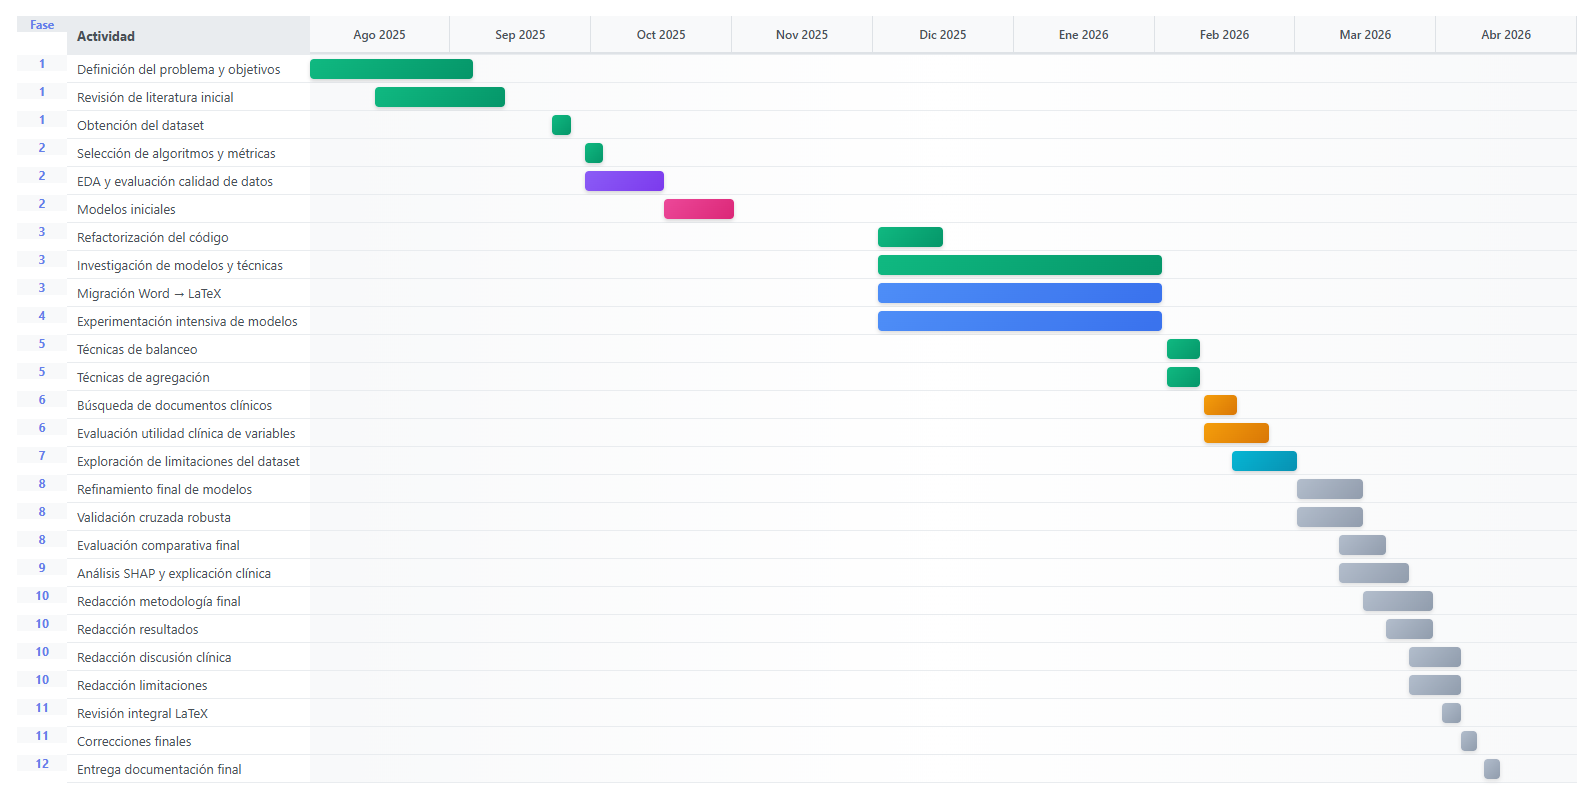
\includegraphics[width=\textwidth]{images/image025.png}
\caption{Cronograma detallado del Proyecto de Grado en Inteligencia Artificial, elaborado mediante TeamGantt}
\end{figure}

\subsection*{Análisis de Participación}
\addcontentsline{toc}{subsection}{Análisis de Participación}

\begin{itemize}
    \item Gustavo Adolfo Cruz Suarez -- Médico Anestesiólogo (FVL)
    \item Daniela Hincapié -- Médico Centro de Investigaciones Clínicas (FVL)
    \item Felipe Ocampo Osorio -- Director de IA (FVL)
\end{itemize}

\newpage

% -----------------------------------------------------------------------------
% ANEXO: EVOLUCIÓN DE EXPERIMENTOS
% -----------------------------------------------------------------------------
\subsection*{Evolución de Experimentos}
\addcontentsline{toc}{subsection}{Evolución de Experimentos}

Se realizaron cinco experimentos para optimizar la predicción del shock hemorrágico. A continuación se presenta la evolución de los modelos evaluados, destacando las mejoras progresivas en AUC-ROC.

\subsubsection*{Experimento 1: Modelos Base}

\textbf{Descripción:} Evaluación inicial de siete algoritmos de machine learning con el conjunto de datos original.

\textbf{Mejor modelo:} \expOneBestModel

\textbf{AUC-ROC (CV):} \expOneAUC

\textbf{Resultados comparativos:}

\begin{figure}[H]
\centering

\includegraphics[width=0.85\textwidth]{../experiments/exp_01_base_models/comparison_plots/roc_comparison.png}
\caption{Comparación de curvas ROC - Experimento 1}
\end{figure}

\subsubsection*{Experimento 2: Características Agregadas}

\textbf{Descripción:} Introducción de variables derivadas: EDAD\textsuperscript{2}, HB\_x\_SANGRADO, síndromes agregados (cardiovascular, metabólico, pulmonar).

\textbf{Mejor modelo:} \expTwoBestModel

\textbf{AUC-ROC (CV):} \expTwoAUC

\textbf{Mejora respecto al Experimento 1:} +0.0082

\begin{figure}[H]
\centering

\includegraphics[width=0.85\textwidth]{../experiments/exp_02_aggregated_features/comparison_plots/roc_comparison.png}
\caption{Comparación de curvas ROC - Experimento 2}
\end{figure}

\subsubsection*{Experimento 3: Características Categóricas}

\textbf{Descripción:} Categorización de variables continuas (EDAD, HB\_PREQX) en rangos clínicos.

\textbf{Mejor modelo:} \expThreeBestModel

\textbf{AUC-ROC (CV):} \expThreeAUC

\textbf{Resultado:} Disminución de rendimiento (-0.0101 vs Exp 2), confirmando que la categorización reduce la precisión predictiva.

\begin{figure}[H]
\centering

\includegraphics[width=0.85\textwidth]{../experiments/exp_03_categorical_features/comparison_plots/roc_comparison.png}
\caption{Comparación de curvas ROC - Experimento 3}
\end{figure}

\subsubsection*{Experimento 4: Poda de Características}

\textbf{Descripción:} Selección de características basada en importancia (eliminación de variables con bajo impacto predictivo).

\textbf{Mejor modelo:} \expFourBestModel

\textbf{AUC-ROC (CV):} \expFourAUC

\textbf{Mejora respecto al Experimento 3:} +0.0075

\begin{figure}[H]
\centering

\includegraphics[width=0.85\textwidth]{../experiments/exp_04_feature_pruning/comparison_plots/roc_comparison.png}
\caption{Comparación de curvas ROC - Experimento 4}
\end{figure}

\subsubsection*{Experimento 5: Búsqueda de Hiperparámetros (Modelo Campeón)}

\textbf{Descripción:} Optimización exhaustiva de hiperparámetros mediante GridSearchCV para todos los modelos.

\textbf{Mejor modelo:} \championModelName

\textbf{AUC-ROC (CV):} \championROCAUC

\textbf{Mejora respecto al Experimento 1:} +0.0238 (mejora del 3.9\%)

\begin{figure}[H]
\centering

\includegraphics[width=0.85\textwidth]{../experiments/exp_05_hyperparameter_search/comparison_plots/roc_comparison.png}
\caption{Comparación de curvas ROC - Experimento 5 (Modelo Campeón)}
\end{figure}

\subsubsection*{Métricas del Modelo Campeón (Conjunto de Prueba)}

El modelo \championModelName\ del Experimento 5 fue seleccionado como modelo campeón por presentar el mejor balance entre Recall (\championRecall) y F2-Score (\championFTwoScore).

\begin{table}[H]
\centering
\caption{Métricas del Modelo Campeón - \championModelName\ (Experimento 5)}
\begin{tabular}{|l|r|}
\hline
\textbf{Métrica} & \textbf{Valor} \\ \hline
AUC-ROC (CV) & \championROCAUC \\ \hline
Brier Score & \championBrierScore \\ \hline
Recall (Sensibilidad) & \championRecall \\ \hline
Especificidad & \championSpecificity \\ \hline
Precisión & \championPrecision \\ \hline
Valor Predictivo Negativo (NPV) & \championNPV \\ \hline
F1-Score & \championFOneScore \\ \hline
F2-Score & \championFTwoScore \\ \hline
Accuracy & \championAccuracy \\ \hline
Kappa de Cohen & \championKappa \\ \hline
Umbral Óptimo & \championOptimalThreshold \\ \hline
\end{tabular}
\end{table}

\textbf{Interpretación clínica:}

\begin{itemize}
    \item \textbf{Recall de \championRecall:} El modelo detecta \championTPpct\% de los casos de shock hemorrágico, cumpliendo el objetivo de maximizar la detección temprana.

    \item \textbf{NPV de \championNPV:} Cuando el modelo predice ausencia de shock, tiene una confianza del \championNPV, lo cual es crucial para reducir intervenciones innecesarias.

    \item \textbf{Especificidad de \championSpecificity:} La baja especificidad implica una tasa de falsos positivos del \championFPpct\%, lo que debe ser comunicado al equipo clínico para evitar fatiga de alertas.

    \item \textbf{F2-Score de \championFTwoScore:} Métrica que pondera más el Recall que la Precisión, alineada con el objetivo clínico de priorizar la detección de casos positivos.
\end{itemize}

\subsubsection*{Características Más Importantes}

Las tres variables con mayor importancia predictiva en el modelo campeón son:

\begin{enumerate}
    \item \textbf{\topFeatureOne:} \topFeatureOneImportance\%
    \item \textbf{\topFeatureTwo:} \topFeatureTwoImportance\%
    \item \textbf{\topFeatureThree:} \topFeatureThreeImportance\%
\end{enumerate}

\begin{figure}[H]
\centering

\includegraphics[width=0.85\textwidth]{../experiments/exp_05_hyperparameter_search/models/xgboost/plots/feature_importance.png}
\caption{Importancia de características - Modelo Campeón (\championModelName)}
\end{figure}

\subsubsection*{Curvas de Calibración}

\begin{figure}[H]
\centering

\includegraphics[width=0.85\textwidth]{../experiments/exp_05_hyperparameter_search/models/xgboost/plots/calibration_curve_cv.png}
\caption{Curva de calibración - Modelo Campeón}
\end{figure}

\subsubsection*{Matriz de Confusión}

\begin{figure}[H]
\centering

\includegraphics[width=0.85\textwidth]{../experiments/exp_05_hyperparameter_search/models/xgboost/plots/confusion_matrix_normalized.png}
\caption{Matriz de confusión - Modelo Campeón (Umbral: \championOptimalThreshold)}
\end{figure}

% Auto-generated annex from experiment metadata JSON
\subsection*{Anexo tecnico de metricas por modelo}
\addcontentsline{toc}{subsection}{Anexo tecnico de metricas por modelo}
Este anexo consolida metricas detalladas por modelo y experimento, variables descartadas en pruning, hiperparametros optimos de la fase 5, importancia de caracteristicas en fases 2 y 3, y el arbol de decision final.

\subsubsection*{Experimento 1 (Baseline): metricas detalladas}
\begin{table}[H]
\centering
\caption{Resumen de discriminacion y calibracion - Experimento 1 (Baseline)}
\scriptsize
\begin{tabular}{|l|c|c|c|}
\hline
\textbf{Modelo} & \textbf{AUC-ROC CV} & \textbf{Brier} & \textbf{Threshold} \\ \hline
catboost & 0.6153 & 0.2134 & 0.2200 \\ \hline
decision\_tree & 0.5557 & 0.3836 & 0.2000 \\ \hline
lightgbm & 0.5943 & 0.2394 & 0.2000 \\ \hline
logistic\_regression\_lasso & 0.6055 & 0.2122 & 0.2500 \\ \hline
naive\_bayes & 0.5713 & 0.5993 & 0.2500 \\ \hline
random\_forest & 0.5856 & 0.2444 & 0.2000 \\ \hline
xgboost & 0.5950 & 0.2476 & 0.2000 \\ \hline
\end{tabular}
\end{table}
\begin{table}[H]
\centering
\caption{Resumen de punto operativo - Experimento 1 (Baseline)}
\scriptsize
\begin{tabular}{|l|c|c|c|c|}
\hline
\textbf{Modelo} & \textbf{Recall} & \textbf{Specificity} & \textbf{F1} & \textbf{Kappa} \\ \hline
catboost & 0.8090 & 0.2991 & 0.4911 & 0.0806 \\ \hline
decision\_tree & 0.4111 & 0.6909 & 0.3995 & 0.1002 \\ \hline
lightgbm & 0.6897 & 0.4330 & 0.4771 & 0.0993 \\ \hline
logistic\_regression\_lasso & 0.8196 & 0.2991 & 0.4960 & 0.0883 \\ \hline
naive\_bayes & 0.8594 & 0.1564 & 0.4713 & 0.0111 \\ \hline
random\_forest & 0.7056 & 0.4093 & 0.4770 & 0.0917 \\ \hline
xgboost & 0.7003 & 0.4606 & 0.4925 & 0.1315 \\ \hline
\end{tabular}
\end{table}

\subsubsection*{Experimento 2 (Agregaciones): metricas detalladas}
\begin{table}[H]
\centering
\caption{Resumen de discriminacion y calibracion - Experimento 2 (Agregaciones)}
\scriptsize
\begin{tabular}{|l|c|c|c|}
\hline
\textbf{Modelo} & \textbf{AUC-ROC CV} & \textbf{Brier} & \textbf{Threshold} \\ \hline
catboost & 0.6192 & 0.2133 & 0.2200 \\ \hline
decision\_tree & 0.5592 & 0.3816 & 0.2000 \\ \hline
lightgbm & 0.5995 & 0.2388 & 0.2000 \\ \hline
logistic\_regression\_lasso & 0.6055 & 0.2122 & 0.2500 \\ \hline
naive\_bayes & 0.5657 & 0.5986 & 0.5000 \\ \hline
random\_forest & 0.5907 & 0.2421 & 0.5000 \\ \hline
xgboost & 0.6045 & 0.2453 & 0.2000 \\ \hline
\end{tabular}
\end{table}
\begin{table}[H]
\centering
\caption{Resumen de punto operativo - Experimento 2 (Agregaciones)}
\scriptsize
\begin{tabular}{|l|c|c|c|c|}
\hline
\textbf{Modelo} & \textbf{Recall} & \textbf{Specificity} & \textbf{F1} & \textbf{Kappa} \\ \hline
catboost & 0.8143 & 0.3091 & 0.4939 & 0.0854 \\ \hline
decision\_tree & 0.4058 & 0.6921 & 0.3943 & 0.0964 \\ \hline
lightgbm & 0.7029 & 0.4318 & 0.4813 & 0.1045 \\ \hline
logistic\_regression\_lasso & 0.8064 & 0.2929 & 0.4880 & 0.0738 \\ \hline
naive\_bayes & -- & -- & -- & -- \\ \hline
random\_forest & -- & -- & -- & -- \\ \hline
xgboost & 0.6843 & 0.4631 & 0.4817 & 0.1211 \\ \hline
\end{tabular}
\end{table}

\subsubsection*{Experimento 3 (Categorizaciones): metricas detalladas}
\begin{table}[H]
\centering
\caption{Resumen de discriminacion y calibracion - Experimento 3 (Categorizaciones)}
\scriptsize
\begin{tabular}{|l|c|c|c|}
\hline
\textbf{Modelo} & \textbf{AUC-ROC CV} & \textbf{Brier} & \textbf{Threshold} \\ \hline
catboost & 0.6134 & 0.2148 & 0.2200 \\ \hline
decision\_tree & 0.5570 & 0.3836 & 0.2000 \\ \hline
lightgbm & 0.5934 & 0.2392 & 0.2000 \\ \hline
logistic\_regression\_lasso & 0.6037 & 0.2125 & 0.2500 \\ \hline
naive\_bayes & 0.5741 & 0.5972 & 0.2900 \\ \hline
random\_forest & 0.5813 & 0.2452 & 0.2000 \\ \hline
xgboost & 0.5950 & 0.2476 & 0.2000 \\ \hline
\end{tabular}
\end{table}
\begin{table}[H]
\centering
\caption{Resumen de punto operativo - Experimento 3 (Categorizaciones)}
\scriptsize
\begin{tabular}{|l|c|c|c|c|}
\hline
\textbf{Modelo} & \textbf{Recall} & \textbf{Specificity} & \textbf{F1} & \textbf{Kappa} \\ \hline
catboost & 0.8143 & 0.2979 & 0.4932 & 0.0835 \\ \hline
decision\_tree & 0.4058 & 0.7046 & 0.3995 & 0.1095 \\ \hline
lightgbm & 0.7003 & 0.4293 & 0.4813 & 0.1045 \\ \hline
logistic\_regression\_lasso & 0.8090 & 0.3004 & 0.4915 & 0.0816 \\ \hline
naive\_bayes & 0.8568 & 0.1640 & 0.4722 & 0.0145 \\ \hline
random\_forest & 0.7109 & 0.4005 & 0.4794 & 0.0947 \\ \hline
xgboost & 0.7003 & 0.4606 & 0.4925 & 0.1315 \\ \hline
\end{tabular}
\end{table}

\subsubsection*{Experimento 4 (Pruning): metricas detalladas}
\begin{table}[H]
\centering
\caption{Resumen de discriminacion y calibracion - Experimento 4 (Pruning)}
\scriptsize
\begin{tabular}{|l|c|c|c|}
\hline
\textbf{Modelo} & \textbf{AUC-ROC CV} & \textbf{Brier} & \textbf{Threshold} \\ \hline
catboost & 0.6237 & 0.2126 & 0.2300 \\ \hline
decision\_tree & 0.5598 & 0.3795 & 0.2000 \\ \hline
lightgbm & 0.5995 & 0.2388 & 0.2000 \\ \hline
logistic\_regression\_lasso & 0.6067 & 0.2111 & 0.2500 \\ \hline
naive\_bayes & 0.5699 & 0.2649 & 0.2000 \\ \hline
random\_forest & 0.5847 & 0.2438 & 0.2000 \\ \hline
xgboost & 0.6038 & 0.2462 & 0.2000 \\ \hline
\end{tabular}
\end{table}
\begin{table}[H]
\centering
\caption{Resumen de punto operativo - Experimento 4 (Pruning)}
\scriptsize
\begin{tabular}{|l|c|c|c|c|}
\hline
\textbf{Modelo} & \textbf{Recall} & \textbf{Specificity} & \textbf{F1} & \textbf{Kappa} \\ \hline
catboost & 0.8011 & 0.3342 & 0.4996 & 0.1024 \\ \hline
decision\_tree & 0.4271 & 0.6859 & 0.4081 & 0.1102 \\ \hline
lightgbm & 0.7029 & 0.4418 & 0.4863 & 0.1173 \\ \hline
logistic\_regression\_lasso & 0.8249 & 0.2628 & 0.4988 & 0.0883 \\ \hline
naive\_bayes & 0.6711 & 0.3917 & 0.4534 & 0.0501 \\ \hline
random\_forest & 0.7162 & 0.4043 & 0.4809 & 0.0957 \\ \hline
xgboost & 0.6897 & 0.4719 & 0.4906 & 0.1329 \\ \hline
\end{tabular}
\end{table}

\subsubsection*{Experimento 5 (Hiperparametros): metricas detalladas}
\begin{table}[H]
\centering
\caption{Resumen de discriminacion y calibracion - Experimento 5 (Hiperparametros)}
\scriptsize
\begin{tabular}{|l|c|c|c|}
\hline
\textbf{Modelo} & \textbf{AUC-ROC CV} & \textbf{Brier} & \textbf{Threshold} \\ \hline
catboost & 0.6215 & 0.2083 & 0.2400 \\ \hline
decision\_tree & 0.6354 & 0.2117 & 0.2200 \\ \hline
lightgbm & 0.6384 & 0.2063 & 0.2400 \\ \hline
logistic\_regression\_lasso & 0.6068 & 0.2396 & 0.4200 \\ \hline
naive\_bayes & 0.5707 & 0.2598 & 0.2000 \\ \hline
random\_forest & 0.6404 & 0.2289 & 0.3800 \\ \hline
xgboost & 0.6371 & 0.2070 & 0.2400 \\ \hline
\end{tabular}
\end{table}
\begin{table}[H]
\centering
\caption{Resumen de punto operativo - Experimento 5 (Hiperparametros)}
\scriptsize
\begin{tabular}{|l|c|c|c|c|}
\hline
\textbf{Modelo} & \textbf{Recall} & \textbf{Specificity} & \textbf{F1} & \textbf{Kappa} \\ \hline
catboost & 0.8488 & 0.2716 & 0.5004 & 0.0880 \\ \hline
decision\_tree & 0.8568 & 0.3154 & 0.5180 & 0.1280 \\ \hline
lightgbm & 0.8700 & 0.2278 & 0.4962 & 0.0700 \\ \hline
logistic\_regression\_lasso & 0.8037 & 0.3191 & 0.4951 & 0.0924 \\ \hline
naive\_bayes & 0.6897 & 0.3554 & 0.4514 & 0.0353 \\ \hline
random\_forest & 0.8196 & 0.3567 & 0.5150 & 0.1344 \\ \hline
xgboost & 0.8594 & 0.3004 & 0.5143 & 0.1180 \\ \hline
\end{tabular}
\end{table}

\subsubsection*{Experimento 5 (Hiperparametros): calibracion comparativa}

La calibracion probabilistica mide la concordancia entre las probabilidades predichas y las frecuencias observadas. La metrica Brier (rango 0-1, menor es mejor) cuantifica el error cuadratico medio entre predicciones y outcomes binarios. Valores cercanos a 0 indican predicciones bien calibradas.

\begin{table}[H]
\centering
\caption{Metricas de calibracion - Top 4 modelos Experimento 5}
\scriptsize
\begin{tabular}{|l|c|c|}
\hline
\textbf{Modelo} & \textbf{Brier Score} & \textbf{Interpretacion} \\ \hline
xgboost & 0.2070 & Mejor calibracion (error cuadratico bajo) \\ \hline
lightgbm & 0.2063 & Calibracion optima \\ \hline
catboost & 0.2083 & Calibracion competitiva \\ \hline
decision\_tree & 0.2117 & Calibracion aceptable \\ \hline
random\_forest & 0.2289 & Calibracion moderada \\ \hline
\end{tabular}
\end{table}

\textbf{Analisis:} Aunque random\_forest lidera en AUC-ROC (0.6404), lightgbm y xgboost presentan mejor calibracion probabilistica (Brier $\approx$ 0.206-0.207). Decision\_tree mantiene calibracion aceptable (0.2117) con maxima interpretabilidad. El trade-off entre discriminacion (AUC) y calibracion (Brier) sugiere que random\_forest prioriza separacion de clases sobre precision probabilistica.

\subsubsection*{Experimento 5 (Hiperparametros): parametros optimos por modelo}
\begin{table}[H]
\centering
\caption{Parametros optimos (optimized\_params) en Experimento 5}
\scriptsize
\begin{tabular}{|l|p{10.5cm}|}
\hline
\textbf{Modelo} & \textbf{Parametros optimos} \\ \hline
catboost & verbose=0, iterations=100, learning\_rate=0.01, depth=5, l2\_leaf\_reg=1, auto\_class\_weights=None \\ \hline
decision\_tree & max\_depth=7, min\_samples\_split=10, min\_samples\_leaf=20, criterion=gini, class\_weight=None \\ \hline
lightgbm & verbosity=-1, n\_estimators=100, learning\_rate=0.01, max\_depth=5, num\_leaves=31, min\_child\_samples=20, subsample=1, colsample\_bytree=1, scale\_pos\_weight=2 \\ \hline
logistic\_regression\_lasso & penalty=l2, solver=lbfgs, max\_iter=10000, C=0.001, class\_weight=None \\ \hline
naive\_bayes & var\_smoothing=0.1 \\ \hline
random\_forest & n\_jobs=-1, n\_estimators=300, max\_depth=5, min\_samples\_split=10, min\_samples\_leaf=20, max\_features=None, class\_weight=balanced \\ \hline
xgboost & verbosity=0, n\_estimators=500, max\_depth=7, learning\_rate=0.01, subsample=1, colsample\_bytree=0.6, scale\_pos\_weight=3, gamma=5, reg\_alpha=0, reg\_lambda=1 \\ \hline
\end{tabular}
\end{table}

\subsubsection*{Importancia de caracteristicas por modelo (Experimentos 2, 3 y 5)}
Para cada modelo se reporta el top 3 de importancia cuando el artefacto esta disponible en \texttt{plot\_metadata.json}. En modelos sin importancia embebida se marca como No aplica.
\begin{table}[H]
\centering
\caption{Top 3 de importancia de caracteristicas en Experimentos 2, 3 y 5}
\scriptsize
\begin{tabular}{|l|l|p{8.5cm}|}
\hline
\textbf{Experimento} & \textbf{Modelo} & \textbf{Top 3 caracteristicas (pct)} \\ \hline
Experimento 2 (Agregaciones) & catboost & HB\_PREQX (26.83\%), EDAD2 (21.34\%), EDAD (20.75\%) \\ \hline
Experimento 2 (Agregaciones) & decision\_tree & HB\_PREQX (35.30\%), EDAD (22.49\%), EDAD2 (16.24\%) \\ \hline
Experimento 2 (Agregaciones) & lightgbm & HB\_PREQX (44.60\%), EDAD (39.07\%), GENERO (3.43\%) \\ \hline
Experimento 2 (Agregaciones) & random\_forest & HB\_PREQX (40.91\%), EDAD (20.64\%), EDAD2 (19.43\%) \\ \hline
Experimento 2 (Agregaciones) & xgboost & SANGRADO\_MAYOR (26.68\%), HIPERTENSION (7.11\%), ACT\_FISICA\_METS (6.08\%) \\ \hline
Experimento 3 (Categorizaciones) & catboost & EDAD (36.92\%), HB\_PREQX (24.89\%), SANGRADO\_MAYOR (9.03\%) \\ \hline
Experimento 3 (Categorizaciones) & decision\_tree & EDAD (38.69\%), HB\_PREQX (36.01\%), GENERO (5.87\%) \\ \hline
Experimento 3 (Categorizaciones) & lightgbm & HB\_PREQX (45.03\%), EDAD (42.43\%), GENERO (3.37\%) \\ \hline
Experimento 3 (Categorizaciones) & random\_forest & EDAD (38.72\%), HB\_PREQX (36.36\%), SANGRADO\_MAYOR (4.20\%) \\ \hline
Experimento 3 (Categorizaciones) & xgboost & SANGRADO\_MAYOR (28.88\%), CANCER\_ACTIVO (9.05\%), HIPOTIROIDISMO (7.64\%) \\ \hline
Experimento 5 (Hiperparametros) & random\_forest & EDAD (52.71\%), HB\_PREQX (27.93\%), SANGRADO\_MAYOR (15.36\%) \\ \hline
Experimento 5 (Hiperparametros) & decision\_tree & EDAD (49.66\%), HB\_PREQX (24.51\%), SANGRADO\_MAYOR (24.19\%) \\ \hline
Experimento 5 (Hiperparametros) & lightgbm & EDAD (52.25\%), HB\_PREQX (36.59\%), SANGRADO\_MAYOR (7.39\%) \\ \hline
Experimento 5 (Hiperparametros) & xgboost & SANGRADO\_MAYOR (30.66\%), EDAD (11.22\%), CARGA\_CARDIOVASCULAR (8.33\%) \\ \hline
\end{tabular}
\end{table}


\newpage


\newpage

\begin{thebibliography}{99}
\addcontentsline{toc}{subsection}{Referencias}

\bibitem{bonanno2023}
F. G. Bonanno, ``Management of Hemorrhagic Shock: Physiology Approach, Timing and Strategies,'' Jan. 01, 2023, MDPI. doi: 10.3390/jcm12010260.

\bibitem{terceros2017}
L. J. Terceros-Almanza et al., ``Prediction of massive bleeding. Shock index and modified shock index,'' \textit{Medicina Intensiva (English Edition)}, vol. 41, no. 9, pp. 532--538, Dec. 2017, doi: 10.1016/J.MEDINE.2017.10.003.

\bibitem{moll2025}
V. Moll, A. K. Khanna, and P. Mathur, ``Artificial intelligence for the prediction of postoperative complications in the critically ill,'' \textit{Critical Care Science}, vol. 37, p. e20250025, 2025, doi: 10.62675/2965-2774.20250025.

\bibitem{hooper2022}
N. Hooper and T. J. Armstrong, ``Hemorrhagic Shock,'' \textit{StatPearls}, Sep. 2022, Accessed: Sep. 07, 2025. [Online]. Available: \url{https://www.ncbi.nlm.nih.gov/books/NBK470382/}

\bibitem{james2023}
G. James, D. Witten, T. Hastie, R. Tibshirani, and J. Taylor, ``An Introduction to Statistical Learning,'' 2023, doi: 10.1007/978-3-031-38747-0.

\bibitem{collins2015}
G. S. Collins, J. B. Reitsma, D. G. Altman, and K. G. M. Moons, ``Transparent reporting of a multivariable prediction model for individual prognosis or diagnosis (TRIPOD): The TRIPOD statement,'' \textit{BMJ (Online)}, vol. 350, Jan. 2015, doi: 10.1136/BMJ.G7594.

\bibitem{zhang2025}
Z. Zhang et al., ``Machine learning model for postpancreaticoduodenectomy haemorrhage prediction: an international multicentre cohort study,'' \textit{BMJ Open}, vol. 15, no. 7, p. e096147, Jul. 2025, doi: 10.1136/BMJOPEN-2024-096147.

\bibitem{cong2025}
X. Cong, X. Zou, R. Zhu, Y. Li, L. Liu, and J. Zhang, ``Development and validation of a machine learning-based model for perioperative stroke prediction in noncardiac, nonvascular, and nonneurosurgical patients,'' \textit{Front Physiol}, vol. 16, p. 1624898, 2025, doi: 10.3389/FPHYS.2025.1624898/FULL.

\bibitem{lucas2019}
A. Lucas, A. T. Williams, and P. Cabrales, ``Prediction of Recovery from Severe Hemorrhagic Shock Using Logistic Regression,'' \textit{IEEE J Transl Eng Health Med}, vol. 7, 2019, doi: 10.1109/JTEHM.2019.2924011.

\bibitem{crispdm1999}
Ncr and J. Clinton, ``CRISP-DM 1.0 Step-by-step data mining guide,'' 1999.

\bibitem{piasta2010}
S. B. Piasta and L. M. Justice, ``Cohen's d Statistic,'' \textit{Encyclopedia of Research Design}, pp. 181--185, May 2010, doi: 10.4135/9781412961288.

\bibitem{wasserstein2016}
R. L. Wasserstein and N. A. Lazar, ``The ASA Statement on p-Values: Context, Process, and Purpose,'' \textit{Am Stat}, vol. 70, no. 2, pp. 129--133, Apr. 2016, doi: 10.1080/00031305.2016.1154108.

\bibitem{allen2017}
M. Allen, ``Cramér's V,'' \textit{The SAGE Encyclopedia of Communication Research Methods}, Jul. 2017, doi: 10.4135/9781483381411.N107.

\bibitem{cannon2018}
J. W. Cannon, ``Hemorrhagic Shock,'' \textit{The New England Journal of Medicine}, vol. 378, no. 4, pp. 370--379, 2018, doi: 10.1056/NEJMra1705649.

\bibitem{ma2023}
J. Ma, P. Dhiman, C. Qi, G. Bullock, M. van Smeden, R. D. Riley, and G. S. Collins, ``Poor handling of continuous predictors in clinical prediction models using logistic regression: A systematic review,'' \textit{Journal of Clinical Epidemiology}, vol. 161, pp. 140--151, 2023, doi: 10.1016/j.jclinepi.2023.07.012.

\bibitem{pal2022}
R. Pal et al., ``ShockModes: A Multimodal Model for Prognosticating Intensive Care Outcomes from Physician Notes and Vitals,'' \textit{medRxiv}, 2022, doi: 10.1101/2022.12.16.22283559.

\bibitem{steyerberg2018}
E. W. Steyerberg, H. Uno, J. P. A. Ioannidis, B. van Calster, and collaborators, ``Clinical prediction models cannot be trusted when common modeling approaches are followed,'' \textit{Journal of Clinical Epidemiology}, vol. 98, pp. 133--143, 2018, doi: 10.1016/j.jclinepi.2018.02.008.

\end{thebibliography}


\end{document}
